\documentclass[twoside]{article}
\usepackage{amssymb}
\usepackage{amsmath}
\usepackage{amsthm}
\usepackage{algorithm}
\usepackage{algpseudocode}
\usepackage{caption}
\usepackage{subcaption}
\usepackage{enumerate}% http://ctan.org/pkg/enumerate
\usepackage{pgfplots}
\usepackage{multicol}
\usepackage[hmarginratio=1:1,top=32mm,columnsep=20pt]{geometry}
\usepackage{fullpage}
\usepackage{pdflscape}
\usepackage{setspace}
\usepackage{url}
\usepackage{tikz}
\usetikzlibrary{tikzmark}
\usepackage{color}
\usepackage{pgfplots}
\usepackage{bm}
\usepackage{tikz-cd}
\pgfplotsset{compat=newest}
\usepgfplotslibrary{fillbetween}
\usepackage[toc,page]{appendix}
\usepackage[shortlabels]{enumitem}\usepackage{draftwatermark}

\usetikzlibrary{arrows.meta,
                calc, chains,
                patterns,
                patterns.meta,
                fit,
                quotes,
                positioning,
                shapes.geometric,
                shapes.misc,
                automata
                }
%Flowchart Tikzset
\tikzset{
   recbox/.style = {
         rectangle,
         draw, 
         align = center, 
         text badly centered,
         inner sep = 6 pt,
         font=\footnotesize,
         line width = 0.3mm,
      },
      circlebox/.style = {
         rounded rectangle,
         draw, 
         align = center, 
         text badly centered,
         inner sep = 7 pt,
         font=\large,
         line width = 0.5mm,
      },
      roundbox/.style = {
         rectangle,
         draw, 
         align = center, 
         rounded corners,
         text badly centered,
         inner sep = 6 pt,
         font=\large,
         line width = 0.5mm,
      },
     box1/.style = {
         rectangle,
         draw, 
         align = center, 
         text badly centered,
         inner sep = 6 pt,
         font=\large,
         line width = 0.5mm,
         minimum width = 30mm,
         minimum height = 7mm,
      },
    papLine/.style = {
         draw,
         -stealth,
         font=\ttfamily,
         line width = 0.5mm,
      },
      }
%end flowcahrt tikz set   

%Colors 
\definecolor{darkgreen}{rgb}{0.01, 0.75, 0.24}
\definecolor{shaded_green}{RGB}{151, 194, 157}

\newcommand{\quotes}[1]{``#1''}

\theoremstyle{plain}% default
\newtheorem{theorem}{Theorem}[section]
\newtheorem{lemma}[theorem]{Lemma}
\newtheorem{proposition}[theorem]{Proposition}
\newtheorem*{corollary}{Corollary}

\theoremstyle{definition}
\newtheorem{definition}{Definition}[section]
\newtheorem{example}{Example}[section]
\newtheorem{exercise}[example]{Exercise}

\theoremstyle{remark}
\newtheorem*{rem}{Remark}
\newtheorem*{note}{Note}
\newtheorem{case}{Case}

\begin{document}
\parindent=0in
\parskip=12pt

\SetWatermarkText{Draft}
\SetWatermarkScale{5}

\title{
  Relative Probability on Finite Sample Spaces \\
  \large{
    SUBTITLE HERE
  }
}

\author{Max Sklar\\ Local Maximum Labs \\ DATE HERE}
\date{}

\maketitle
\thispagestyle{empty}

\begin{abstract}
This is an incomplete draft/outline of an upcoming paper. Please do not share
\end{abstract}

\tableofcontents
\newpage

\section{Introduction}

The foundations of probability theory are still very much open to debate!

Since Kolmogorov published the standard axioms for probability\cite{kolmogorov} in 1933, there have been calls to relax or alter them for various applications. In Kolmogorov's Axiomatisation and Its Discontents\cite{lyon}, Lyon lays out these cases and their justifications.
One controversy concerns conditional probability. We talk about \quotes{the probability of A given that B occured} and denote it as \(P(A|B)\) - but can this make sense if \(B\) never occurs (or has probability zero\footnote{Another unintuitive feature of probability theory is that zero probability events do indeed occur, particularly when given a continuous distribution.})? We are out of luck if we stick to the Kolmogorov model, which defines the conditional probability above as the ratio \(\frac{P(A \cap B)}{P(B)}\). If the probability of B is zero, the indeterminate form \(\frac{0}{0}\) appears.

Undeterred, mathematicians and engineers refer to this type relative probability all the time. For example, if we consider a continuous probability distributrion over \([0, 1]\) given by the probability distribution function \(2x\), we know that the PDF at \(x = \frac{1}{2}\) is twice as much as the PDF at \(x = \frac{1}{4}\). In a sense, we believe that the former is twice as likely as the latter - even though we are only talking about \textit{probability density}. Hajek\cite{hajek} (citing Borel) gives a much more compelling example: if a random point on the Earth is selected, what is the probability that it is in the eastern hemisphere given that it is on the equator? Most people would not hesitate to answer one half, and yet the equator - being a mere 1-dimentional object - has probability 0 compared to the rest of the globe.

Let us take the position that we may model probability in a non-standard way, and we can do so as long our new framework is logically consistent, and the advertised applications correspond to the new model\footnote{Lyon identifies this link between application and model as the bridge principle. A new set of axioms for probability could well give rise to a new and interesting mathematics, but if that mathematics cannot be linked to any application that anyone would reasonbly call probability, then it ought to go by a different name.}. We ought to understand whether we can derive a framework for probability that takes the relationships between outcomes and events as the fundamental unit.

This improves the Kolmogorov model - that starts with an absolute probability function - by both solving the conditional probability question and giving rise to new objects and patterns to study. 

\subsection{Goals}

The relative approach to probability is not only viable, but has many properties that practicioners will find attractive. For example, many Bayesian inference algorithms rely on relative probability alone to search for optimal parameters. 

As a proof of this concept, we will construct a theory of relative probability on finite distributions. By omitting infinite distributions, we temporarily set aside the concepts of measurable sets and countable additivity\footnote{In the textbook Invitation to Discrete Mathematics, Matoušek et al. write \quote{By restricting ourselves to finite probability spaces we have simplified the situation considerably... A true probability theorist would probability say that we have excluded everything interesting.}}. This work will demonstrate that even with this vast simplification there is much to be learned. Relative probability requires a new set of fundamental rules and vocabulary, which we will construct without the distractions of infinite and continuous outcome spaces.

We then provide a new formulation of Bayes rule that uses only relative proability, and that is reflective of current practice. We will look at these applications of these ideas along with their algorithmic implementation.

Finally, we discuss a critical feature of relative probability functions,
which is their ability to retain information when taking limits\textemdash for which absolute probability fails. To that end, we delve into the topology of the relative probability space, and finish with a proof of compactness.

\subsection{Previous Work}
Mention the work of heinemann\cite{heinemann} and previous work on condition probability spaces.

\section{Preliminaries}
\subsection{Magnitude Space}

\begin{definition}
The \textit{magnitude space} \(\mathbb{M}\) is the set of all positive real numbers, \(0\) and \(\infty\).
\[\mathbb{M} = [0, +\infty]\]
\end{definition}

Magnitudes correspond with our intuition of size. Unlike the set of non-negative real numbers, magnitudes include a point at infinity. The point at infinity can be considered a limit element, larger that all of the other magnitudes. It provides the magnitude space with several important properties.

\begin{enumerate}
\item \(Compactness:\) sequences that go off to infinity still a limit (at \(\infty\)).
\item Symmetry around ratios: When we compare the probability of two events, we get their \textit{odds}. If the odds are 0, then we are comparing an event with probability 0 to an event with probability > 0. We should be able to reverse this comparison, and talk about it from either side. If we're comparing the probability of an event to its converse, then \(\infty\) represents events that have probability 1.
\item Actual measurement value: Whereas physical objects may not be able to have infinite size, mathematical objects do. The infinite element is introduced in measure theory because many mathematical systems (real and natural numbers for example) contain sets of infinite measure.
\end{enumerate}

We set \(0^{-1} := \infty\) and \(\infty^{-1} := 0\), even though their product is indeterminate.

\subsection{The Wildcard Element}

\begin{definition}
Let the \textit{magnitude-wildcard space} \(\mathbb{M}^*= \mathbb{M} \cup \{\ast\}\) be the set of magnitudes along with a \textit{wildcard element}, \(\ast\).
\end{definition}

The wildcard element corresponds to several different concepts, each appearing in a different type of practice:
\begin{itemize}
  \item The \textit{NaN}, or \textit{Not a Number}\footnote{\quotes{Not a Number} may have been an unfortunate naming choice because it actually represents \textbf{any} number!} value in the IEEE standard for floating point arithmetic\cite{ieee}.
  \item The indeterminate form \(\frac{0}{0}\) in arithmetic.
  \item The \textit{wildcard pattern} used in pattern matching and regular expressions in type theory and computer science
\end{itemize}

The following properties on \(\ast\) to allow addition and multiplication of any two magnitude-wildcard values.
\begin{enumerate}[(i)]
  \item \(0 \cdot \infty = \ast\)
  \item \(\ast + m = \ast\)
  \item \(\ast \cdot m = \ast\)
\end{enumerate}

Unfortunately, we now lose some basic algebraic properties: we can no longer simplfy an expression like \(0x\) to \(0\) for example. This will take some getting used to, but programmers familiar with the floating point value \textit{NaN} have long adapted to this.

\subsection{The Matching Relation}

\begin{definition}
The \textit{matching relation}\footnote{It helps to read \(:\cong\) as \quotes{is matched by}.} \(:\cong\) is a binary relation on \(\mathbb{M}^*\). \(m_1\) is matched by \(m_2\) when either \(m_1 = m_2\) or  \(m_2\) is the wildcard.
\[m_1 :\cong m_2 \Longleftrightarrow (m_1 = m_1) \vee (m_2 = \ast)\]
\end{definition}

The left hand side of a matching relation is the \textit{parameter} and the right hand side is the \textit{constraint}. This reinforces the idea that the \(contraint\) may or may not constrain the parameter. The wildcard element represents every single value, but it cannot be represented by any specific value. Alternatively, the wildcard element also represents a loss of information about a parameter which can never be recovered.

The following lemmas quickly follow from the definition.

\begin{lemma}
\label{wild_prop_1} If a magnitude matches a non-wildcard element, then the two values are equal. \[m_1 :\cong m_2 \wedge m_2 \neq \ast \Longrightarrow m_1 = m_2\]
\end{lemma}

\begin{lemma}
\label{wild_prop_2}
Every element is matched by the wildcard element. \(m :\cong \ast\)
\end{lemma}

\begin{lemma}
\label{wild_prop_3}
The wildcard element is matched only by itself. \(\ast :\cong m \Longrightarrow m = \ast\)
\end{lemma}

The matching relation looks a lot like equality, and in many cases it is, but because of the introduction of the wildcard it doesn't always act in the same way.

\begin{theorem}
The matching relation is reflexive and transitive, but unlike equality is not symmetric.
\end{theorem}

\begin{proof}
Reflexive is obvious: \(m :\cong m \Longleftrightarrow (m = m) \vee (m = \ast)\)

The transitive property states that for all \(m_1, m_2, m_3\) in \(\mathbb{M}\), if \(m_1 :\cong m_2\) and \(m_2 :\cong m_3\), then \(m_1 :\cong m_3\).

Assume that \(m_1 :\cong m_2\) and \(m_2 :\cong m_3\). If none of these values are the wildcards, then by property \ref{wild_prop_1}, they are all equal and \(m_1 :\cong m_3\). If \(m_1 = \ast\) then by property \ref{wild_prop_3}, \(m_2 = \ast\) and finally \(m_3 = \ast\) so the theorem holds. If \(m_2 = \ast\) then \(m_3 = \ast\) and \(m_1 :\cong m_3\) by property \ref{wild_prop_2}. And of course if \(m_3 = \ast\) alone, then by property \ref{wild_prop_2}, \(m_1\) is still matched by \(m_3\).

For non-symmetric, we present a counterexample: \(1 :\ncong \ast\) but \(\ast :\ncong 1\)
\end{proof}

We could also define a symmetric matching relation \(m_1 :\cong: m_2\) to mean \(m_1 :\cong m_2 \vee m_2 :\cong m_1\). This would be symmetric, but not transitive.

\begin{theorem}
\label{theorem:matching_multiplication}
The matching relation preserves multiplication and addition. \(\forall a,b,a',b' \in \mathbb{M^*}\) if \(a :\cong a'\) and \(b :\cong b'\), then \(ab :\cong a'b'\) and \(a+b :\cong a'+b'\).
\end{theorem}

\begin{proof}
For multiplication: Let \(a,b,a',b' \in \mathbb{M^*}\), and let \(a :\cong a'\) and \(b :\cong b'\). If either \(a'\) or \(b'\) are wildcards, then \(a'b'\) is also a wildcard. If \(a'\) and \(b'\) are not wildcards, then \(a = a'\) and \(b = b'\), also making \(ab :\cong a'b'\).
The same argument proves \(a+b :\cong a'+b'\).
\end{proof}

\section{Categorical Distribution}

Let \(\Omega\) be a set of mutually exclusive \textit{outcomes}\footnote{Each outcome could be thought of as a possible result of a random trial, or a possible outcome for an unknown variable}. We assume that \(\Omega\) is finite so that we can count its members as \(|\Omega| = K\). We say there are \(K\) outcomes, or \textit{categories}.

\begin{definition}
\label{def:categorical_abs}
A \textit{categorical distribution} on a \(\Omega\) is a function \(P: \Omega \rightarrow [0, 1]\) such that \(\sum_{h \in \Omega} P(h) = 1\)
\end{definition}

The set of all categorical distributions of size \(K\) can be embedded in \(\mathbb{R}^K\) as a (K-1)-dimentional object called a (K-1)-simplex (see figure \ref{fig:simplex}). For example, if \(K = 3\), the resulting space of categorical distributions is an equilateral triangle embedded in \(\mathbb{R}^3\) connecting the points (1, 0, 0), (0, 1, 0), and (0, 0, 1).

\begin{figure}[h]
\centering
\resizebox{0.3\textwidth}{!}{
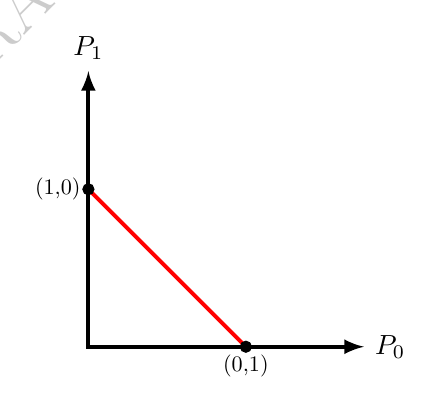
\begin{tikzpicture} %Segment P_0,P_1
\draw[-latex,line width=0.5mm] (0,2)--(0,0) -- (3.5,0) node[right]{\(P_{0}\)};
\draw[-latex,line width=0.5mm] (0,0)--(0,3.5) node[above]{\(P_{1}\)};
\draw[red,line width=0.5mm] (2,0)--(0,2);
\draw[fill=black] (2,0) circle (2pt) node[black,below,scale=0.8] {(0,1)};
\draw[fill=black] (0,2) circle (2pt) node[black,left,scale=0.8] {(1,0)};
\end{tikzpicture}
}
\resizebox{0.3\textwidth}{!}{
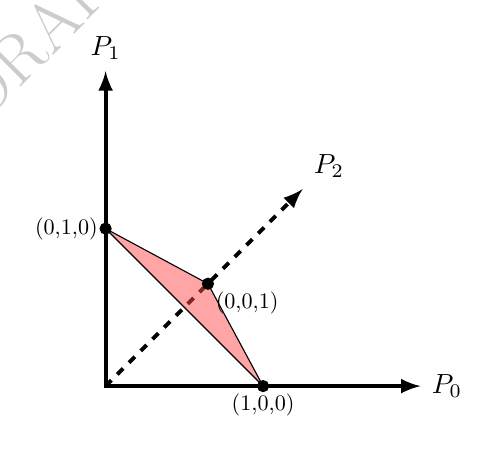
\begin{tikzpicture} %Triangle P_0,P_1,P_2
\draw[-latex,line width=0.5mm] (0,2,0)--(0,0,0) -- (4,0,0) node[right]{\(P_{0}\)};
\draw[-latex,line width=0.5mm] (0,0,0) -- (0,4,0) node[above]{\(P_{1}\)};
\draw[-latex,line width=0.5mm,dashed] (0,0,0) -- (0,0,-6.5) node[above right]{\(P_{2}\)};
\draw[fill=red!70!,fill opacity=0.5] (2,0)--(1.3,1.3)--(0,2)--cycle;
\draw[fill=black] (2,0) circle (2pt) node[black,below,scale=0.8] {(1,0,0)};
\draw[fill=black] (1.3,1.3) circle (2pt) node[black,below right,scale=0.8] {(0,0,1)};
\draw[fill=black] (0,2) circle (2pt) node[black, left,scale=0.8] {(0,1,0)};
\end{tikzpicture}
}
\resizebox{0.3\textwidth}{!}{
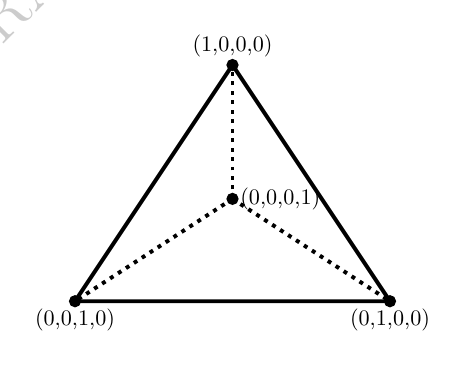
\begin{tikzpicture} %Tetrahedron 
\draw[line width=0.5mm] (0,3)--(-2,0)--(2,0)--cycle;
\draw[line width=0.5mm,dotted] (0,1.3)--(2,0);
\draw[line width=0.5mm,dotted] (0,1.3)--(-2,0);
\draw[line width=0.5mm,dotted] (0,1.3)--(0,3);
\draw[fill=black] (2,0) circle (2pt) node[black,below,scale=0.8] {(0,1,0,0)};
\draw[fill=black] (0,1.3) circle (2pt) node[black,right,rotate=0, scale=0.8] {(0,0,0,1)};
\draw[fill=black] (0,3) circle (2pt) node[black,above,scale=0.8] {(1,0,0,0)};
\draw[fill=black] (-2,0) circle (2pt) node[black,below,scale=0.8] {(0,0,1,0)};
\end{tikzpicture}
}
\caption{An illustration of the probability simplex for K = 2, 3, and 4. These objects are respectively, a segment embedded in \(\mathbb{R}^2\), an equilateral triangle embedded in \(\mathbb{R}^3\), and a normal tetrahedron embedded in \(\mathbb{R}^4\). We make no attempt to visualize the 4D space that contains the tetrahedron.}
\label{fig:simplex}
\end{figure}

With absolute probability, information about relative probability is lost at the vertices where several probabilities might go to zero. For example, if \(\Omega = {a, b, c}\) with \(P(a) = 1\) and \(P(b) = P(c) = 0\), we cannot compare the probabilities of \(b\) and \(c\) as we can in the rest of the simplex.

This poses an interesting problem for limits.

\begin{example}
\label{ex:abs_lose_info}
Consider the following categorical distribution function, with parameter \(\epsilon > 0\):
\[
P(a) = 1 - \epsilon
P(b) = \frac{2}{3}\epsilon
P(c) = \frac{1}{3}\epsilon
\]
\end{example}

This is clearly an absolute probability, and its clear that the limit as \(\epsilon\) goes to zero should be \(P(a) = 1, P(b) = P(c) = 0\). The fact that b is twice as likely as c is lost!

\subsection{Events}

An \textit{event} is a set of outcomes, and by convention \(\mathcal{F}\) is the set of all possible events. \(\mathcal{F}\) is the power set\footnote{In general, \(\mathcal{F}\) is not the entire power set of \(\Omega\) but typically is when \(\Omega\) is finite. We need not concern ourselves with the \(\sigma\)-algebra of measurable sets here.} of \(\Omega\), meaning that \(\mathcal{F} = \mathcal{P}(\Omega)\), and for any subset \(e \subseteq \Omega\), \(e \in \mathcal{F}\).

In the previous section, we defined the probability of individual outcomes. We can now define the probability of an event - that is the probability that any one of its outcomes occur.
Looking at probability on the event level rather than the outcome level is a crucial insight in the development of probability theory (and measure theory more generally). Even though the process is far simpler for finite distributions, we must pay attention to this layer in order for the framework to generalize.

For all \(e\) in \(\mathcal{F}\),
\[ P(e) = \sum_{h \in e}{P(h)}\]

We can take \(P\) as acting either on outcomes or events using the convention \(P(\{h\}) = P(h)\).

\(\Omega\) itself the \textit{universal event} of all outcomes, with probability 1.

\[P(\Omega) = \sum_{h \in \Omega}{P(h)} = 1\]

\subsection{Relative Probability Function}
\label{section:standard_relative_prob}

A \textit{relative probability function}, or \textit{RPF}, measures the probability of one event with respect to another. For example, we may wish to talk about an event that is \quotes{twice as likely} as another, even if we don't know the absolute probability of either event.

We continue to use P to represent the RPF but with two inputs instead of one. The expression \(P(e_1, e_2)\) can be read as the probability of \(e_1\) relative to \(e_2\).

\[P: \mathcal{F} \times \mathcal{F} \rightarrow \mathbb{M}^*\]

We define relative probability in terms of absolute probability as a ratio, in the style of the standard Kolmogorov framework.

\begin{definition}
\label{def:ratio}
The relative probability of events \(e_1\) and \(e_2\) on an categorical distribution \(P\) is given as
\[P(e_1, e_2) = \frac{P(e_1)}{P(e_2)}\]
\end{definition}

If \(P(e_1) = P(e_2) = 0\), then \(P(e_1, e_2) = \ast\), representing the classical problem of zero-probability events being incomparable.

\begin{theorem}[Composition]
For all events \(e_1, e_2, e_3\), \(P(e_1, e_3) :\cong P(e_1, e_2) \cdot P(e_2, e_3)\)
\end{theorem}

\begin{proof}
Start with the case that \(P(e_2)\neq 0\). Then \(P(e_1, e_2) \cdot P(e_2, e_3) = \frac{P(e_1)}{P(e_2)}\frac{P(e_2)}{P(e_3)} = \frac{P(e_1)}{P(e_3)} = P(e_1, e_3)\). When \(P(e_2) = 0\), \(P(e_1, e_2) \cdot P(e_2, e_3) = \frac{P(e_1)}{P(e_2)}\frac{P(e_2)}{P(e_3)} = \ast\). Because \(\ast\) matches everything, then the matching statement holds. Because it holds in both cases, the theorem is true.
\end{proof}

\section{The Relative Probability Approach}
\label{section:new_relative_prob}

In section \ref{section:standard_relative_prob}, the relative probability function was derived from the absolute probability function. Here in section \ref{section:new_relative_prob}, we start with the relative probability function as the fundamental object of study.

\subsection{Fundamental Axioms}

Consider a relative probability function \(P\) that acts on outcomes only.

\begin{definition}
\label{def:fundamental_laws}
Let \(\Omega\) be the set of outcomes, and \(P: \Omega \times \Omega \rightarrow \mathbb{M}^*\) be a function acting on two outcomes to produce a magnitude-wildcard. \(P\) is a \textit{relative probability function on the outcomes of \(\Omega\)} if it obeys the \textit{3 fundamental axioms of relative probability}:

\begin{enumerate}[(i)]
\item The \textit{identity axiom}: \(P(h, h) = 1\)
\item The \textit{inverse axiom}: \(P(h_1, h_2) = P(h_2, h_1)^{-1}\)
\item The \textit{composition axiom}: \(P(h_1, h_3) :\cong P(h_1, h_2) \cdot P(h_2, h_3)\)
\end{enumerate}

\end{definition}

If \(P\) is a relative probability function, \(P(h_1, h_2)\) can be read as the probability of \(h_1\) relative to \(h_2\). Outcomes \(h_1\) and \(h_2\) are said to be \textit{comparable} if \(P(h_1, h_2) \neq \ast\).

Let us pause for a moment to discuss how these axioms where chosen. The star of the show is the composition axiom which succinctly encodes how relative probability works. If \(A\) is twice as likely as \(B\), and \(B\) is 3 times as likely as \(C\), then \(A\) had better be 6 times as likely as \(C\). If it were not, then these relative probability assignments would have no meaning.

The composition axiom is enough to show that the identity axiom works most of the time. For example, if one can compare an outcome \(h_1\) to any other outcome \(h_2\) then through composition we get \(P(h_1, h_2) :\cong P(h_1, h_1) \cdot P(h_1, h_2)\). So long as \(P(h_1, h_2)\) isn't \(0\), \(\infty\), or \(\ast\), then we would have to conclude \(P(h_1, h_1) = 1\).

But that doesn't get us all the way there! We can still construct scenarios where \(P(h, h) = \ast\). Hence, the neccesity of the identity axiom.

Composition and identity can actually be combined into a single axiom about composition paths. It's a bit more unweildy for the mathematical proofs, but nevertheless interesting.

\begin{proposition}[Path Composition]
Given a non-empty list of \(N\) outcomes \(h_0, h_1, h_2, ..., h_{N-1}\), \[P(h_0, h_{N-1}) :\cong \prod_{k=0}^{N-2} P(h_k, h_{k+1}) \]
\end{proposition}

In this case, \(P(h_0, h_0)\) would be matched by the empty product, which is 1.

The inverse axiom is nearly redundant as well. Since \(P(h_0, h_0) \cong P(h_0, h_1) \cdot P(h_1, h_0)\), the terms in the constaint look like they must be inverses! But without stating the axiom explicitly, there could be a case where \(P(h_0, h_1)\) is some non-wildcard magnitude like 2 but \(P(h_1, h_0)\) is not comparable. This shouldn't be allowed because \(\ast\) represents a lack of knowledge about a value, and we consider \(P(h_1, h_0)\) and \(P(h_1, h_0)\) to be the exact same piece of information but in reverse.

\subsection{Examples}

\begin{definition}
\label{def:uniform_rpf}
The \textit{uniform} RPF can be constructed from any number of outcomes where each are considered equally likely. \(P(h_1, h_2) = 1\) for every pair of outcomes.
\end{definition}

\begin{definition}
\label{def:uncomparable_rpf}
The \textit{uncomparable} RPF has \(P(h_1, h_2) = \ast\) for every pair of outcomes. It is as if the subjective probability agent gave up.
\end{definition}

\begin{definition}
A \textit{certain} RPF contains a single outcome that has infinite probability relative to all other outcomes. Let \(h_C\) be the certain outcome with \(h_C \neq h\). Then \(P(h_C, h) = \infty\). The relative probability of the other \(K-1\) outcomes could be anything.
\end{definition}

\begin{definition}
\label{def:empty_rpf}
The \textit{empty} RPF has no outcomes \(K = 0\), and therefore the function \(P\) has no valid inputs.
\end{definition}

It is surprising that there is still an RPF with \(\Omega = \varnothing\).This is an interesting comparison to absolute distributions where such a function does not exist (because with no outcomes, they cannot sum to 1).

\begin{definition}
\label{def:unit_rpf}
The \textit{unit} RPF has a single outcome where \(K = 1\) and \(\Omega = h\). There is only one such RPF where \(P(h, h) = 1\).
\end{definition}

The unit RPF is a special case of the uniform RPF and the certain RPF. This matches the absolute case where the probability of the single outcome must be 1.

\begin{definition}
\label{def:finite_geometric_rpf}
Let \(P\) be an RPF with K outcomes labeled \((h_0, h_1, ..., h_{K-1})\). \(P\) is a \textit{finite geometric} RPF with ratio \(r\) if the relative probabilities of each outcome with its neighbor is always \(r\). In other words, for all \(i \in (0, 1, ..., K-2)\),
\[P(h_{i+1}, h_i) = r\]
When \(r\) is 0 or \(\infty\), we can call this the \textit{limit finite geometric} RPF.
\end{definition}

Finally, to include an example that is both common and has powerful applications, there is a relative version of the Binomial distribution.

\begin{definition}
\label{def:binomial_rpf}
A \textit{binomial distribution} has a sample size we can call \(n\), and a probability of success \(p\). The RPF is uses\(\Omega = \{0, 1, 2, ..., n\}\), and thus \(K = n + 1\). It is given as follows:
\[P(h_1, h_2) = \frac{h_2!(n-h_2)!}{h_1!(n-h_1)!}\left(\frac{p}{1-p}\right)^{h_1 - h_2}\]
\end{definition}


\section{New Concepts for Relative Probability}

We have successfully defined the relative probability in section \ref{section:new_relative_prob} with fundamental axioms and have constructed some examples. Because new situations arise that do not occur in the Kolmogorov model, we need to define some new vocabulary.

Fortunately, we can look at the absolute probability function as a special case of relative probability, defined by \(P(h_1, h_2) = \frac{P(h_1)}{P(h_2)}\).

Figure \ref{fig:flow_chart} gives us a roadmap of these new concepts and their relationship to each other.

\begin{figure}
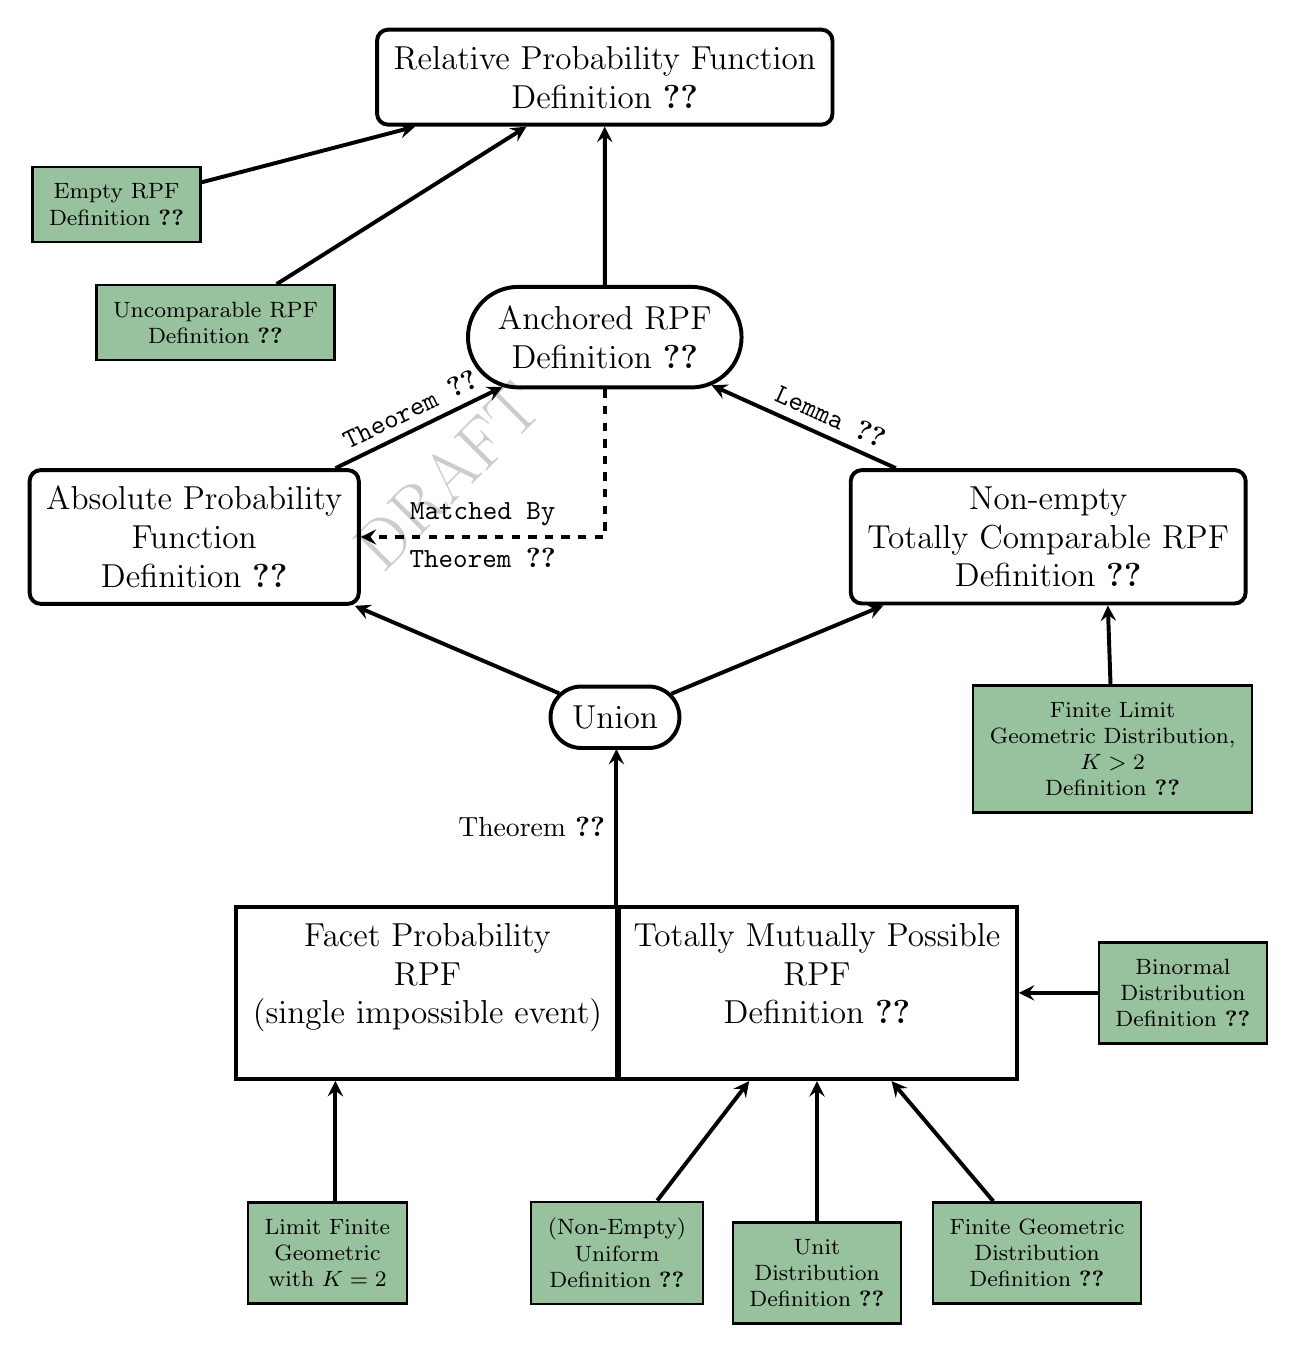
\begin{tikzpicture}    %Flowchart
[node distance = 1.3in] %Node distance

%node0 for Relative Probability Functions
\node (node0) [roundbox] {Relative Probability Function \\ Definition \ref{def:fundamental_laws}} ;

%node1 Anchored RPF
\node (node1) [circlebox, below of=node0] {Anchored RPF\\ Definition \ref{def:anchored_rpf}};

%lnode1 Empty RPF
\node (lnode1) [recbox, fill=shaded_green,below left=0.5 and 2.2 of node0] {Empty RPF\\ Definition \ref{def:empty_rpf}};

%lnode2 Uncomparable RPF
\node (lnode2) [recbox, fill=shaded_green,below left=2 and 0.5 of node0] {Uncomparable RPF\\ Definition \ref{def:uncomparable_rpf}};

%node2 Non-empty Totally Comparable RPF
\node (node2) [roundbox, below right= and 2 of node1] {Non-empty\\ Totally Comparable RPF\\ Definition \ref{def:totally_comparable}};

%bnode2 Finite Limit Geometric Distribution, \(K>2\)
\node (bnode2) [recbox, fill=shaded_green, below right=1 and -3.5 of node2] {Finite Limit \\Geometric Distribution,\\ \(K>2\)\\ Definition \ref{def:finite_geometric_rpf}};

%node3 Absolute Probability\\ Function
\node (node3) [roundbox, below left= and 2 of node1] {Absolute Probability\\ Function\\ Definition \ref{def:categorical_abs}};

%node4 Union
\node (node4) [circlebox, below right=and 2.8 of node3] {Union};

%node5 Facet Probability\\ Functions\\(single impossible event)
\node (node5) [box1, below left=and -0.5 of node4,yshift=-0.38in] {Facet Probability\\ RPF\\(single impossible event)\\};

%node6 Mutually Possible\\ RPFs
\node (node6) [box1, right=-0.07 of node5] {Totally Mutually Possible\\ RPF\\ Definition \ref{def:totally_mutually_possible}\\};

%rnode4 (Non-Empty)\\ Uniform
\node (rnode4) [recbox, fill=shaded_green, below of=node6,xshift=-1.0in,yshift=-0.0in] {(Non-Empty)\\ Uniform\\ Definition \ref{def:uniform_rpf}};

%rnode3 Unit\\ Distribution
\node (rnode3) [recbox, fill=shaded_green, below of=node6,yshift=-0.1in] {Unit\\ Distribution\\ Definition \ref{def:unit_rpf}};

%rnode2 Finite Geometric\\Distribution
\node (rnode2) [recbox, fill=shaded_green, below of=node6,xshift=1.1in,yshift=-0.0in] {Finite Geometric\\Distribution\\ Definition \ref{def:finite_geometric_rpf}};

%rnode1 Binormal\\Distribution
\node (rnode1) [recbox, fill=shaded_green, right=1 of node6] {Binormal\\Distribution\\ Definition \ref{def:binomial_rpf}};

%lnode3 Limit Finite\\Geometry\\ with \(K=2\)
\node (lnode3) [recbox, fill=shaded_green, below of=node5,yshift=-0.0in,xshift=-0.5in] {Limit Finite\\Geometric\\ with \(K=2\)};

%Arrow paths for all nodes
\path[papLine] (rnode1) -- (node6);

\path[papLine] (rnode2) --+ (node6);

\path[papLine] (rnode3) -- (node6);

%\path[papLine] (rnode4) --+(0,0.56in)--+(1in,0.56in)-- +(1in,0.87in); (node6);
\path[papLine] (rnode4) --+ (node6);

\path[papLine] (lnode1) --+ (node0);

\path[papLine] (lnode2) --+ (node0);

\path[papLine] (node1) -- (node0);

\path[papLine] (node2) -- (node1) node[pos=0.4, above, sloped]{Lemma \ref{lemma:totally_comp_anchored}};

\path[papLine] (node3) -- (node1) node[pos=0.5, above, sloped]{Theorem \ref{thm:absolute_anchored}};

\path[papLine] (node4) -- (node3);

\path[papLine] (node4) -- (node2);

\draw[-stealth,transform canvas={xshift=1mm},line width=0.5mm] (lnode3) -- +(0,0.86in);

\draw[-stealth,transform canvas={xshift=24mm},line width=0.5mm] (node5) --+(0,1.22in) node[left,pos=0.5]{Theorem \ref{thm:abs_totally_comparable}};

\path[papLine,dashed] (node1) |- (node3) node[above,pos=0.75]{Matched By} node[below,pos=0.75]{Theorem \ref{thm:absolute_prob_formula}};

\path[papLine] ([xshift=0.6in]bnode2) -- (node2);
\end{tikzpicture}
\caption{This is our roadmap for all of the sub-types of relative probability functions and their relationship to one another. }
\label{fig:flow_chart}
\end{figure}

\subsection{Matching and Comparability}

\begin{definition}
\label{def:totally_comparable}
A relative probability function is \textit{totally comparable} if every pair of outcomes are comparable.
\end{definition}

\begin{theorem}
\label{thm:abs_totally_comparable}
An absolute probability function is totally comparable if and only if \(P(h) = 0\) for at most one outcome.
\end{theorem}

\begin{proof}
Let P be an \textbf{absolute} probability function, with \(h_1\) and \(h_2\) being two outcomes. If \(P(h_1) = P(h_2) = 0\), then \(P(h_1, h_2) = \frac{0}{0} = \ast\). If only outcome \(h_1\) is assigned 0, then \(P(h_1, h_1) = 1\), \(P(h_1, h_2) = 0\), and \(P(h_2, h_1) = \infty\). Any other pairing that does not involve \(h_1\) will be the quotient of two positive numbers, and thus also comparable.
\end{proof}

\begin{definition}
\label{def:anchored_rpf}
An \(anchored\) RPF has at least 1 outcome whose probability relative to every other outcome is greater than zero. We call this outcome an \(anchor\) element, and there may be multiple.
\end{definition}

The anchored concept is useful because it means that every pair of outcomes, even if they are not comparable, are at least going to be 0 compared to a larger outcome. The anchoring of a distribution is important to ensure that it is well behaved.

\begin{theorem}
\label{thm:absolute_anchored}
All absolute probability distributions are anchored.
\end{theorem}

\begin{proof}
Let P be an absolute probability distribution on \(\Omega\). Because \(\sum_{h \in \Omega} P(h) = 1\), there must be at least one \(h\) such that \(P(h) > 0\).  Therefore, for any comparison outcome \(h'\), \(P(h, h') > 0\)
\end{proof}

\begin{lemma}
\label{lemma:totally_comp_anchored}
Every non-empty, totally comparable RPF is anchored.
\end{lemma}

\begin{proof}
Let \(P\) be non-empty and totally comparable RPF. Assume the opposite - that is for every outcome \(h\), there exists another outcome \(h'\) such that P(h, h') = 0.

Therefore, a function \(f: \Omega \rightarrow \Omega\) can be created so that for every \(h\), \(P(h, f(h)) = 0\).

Let \(f^n(h)\) be the function \(f\) applied to \(h\) n times. Then \(P(h, f^n(h)) = 0\) for all n greater than 0. This is by induction because the case of \(n = 1\) was assumed above, and for for inductive step\[P(h, f^{n+1}(h) :\cong P(h, f^n(h)) \cdot P(f^n(h), f(f^n(h)) = 0 \cdot 0 = 0\]

Because \(\Omega\) is finite, repeated applications of \(f\) on \(h\) must evenually return to an outcome that has already been visited. In more rigorous terms, there exists an \(N\) such that \(f^N(h) = f^i(h)\) for some \(i < N\).

But this is a contradiction because \(P(f^i(h), f^N(h))\) should equal 0 by the argument above, but 1 by the identity axiom.
\end{proof}

A totally comparable RPF contains the maximum amount of information about the relative probability of two events. Some RPFs may have less information but nevertheless are consistent with RPFs that have more. The following definition encapulates this relationship.

\begin{definition}
Let \(P_1\) and \(P_2\) be relative probability functions. \(P_1\) is matched by \(P_2\) if and only if all of relative probabilities of \(P_1\) are matched by those of \(P_2\).
\[\forall h_1, h_2 \in \Omega, P_1(h_1, h_2) :\cong P_2(h_1, h_2)\]
\end{definition}

\begin{theorem}
\label{thm:absolute_prob_formula}
Every anchored RPF is matched by an absolute probability function, given by the following equation where \(a\) is an anchor outcome.
\[P(h) = \frac{P(h, a)}{\sum_{h' \in \Omega}P(h', a)}\]
\end{theorem}

\begin{proof}
We need to show that \(P(h)\) is a valid absolute probability function, and that it matches the original RPF.

Because \(a\) is an anchor element, we know that \(P(h', a) < \infty\). This means that the sum \(\sum_{h' \in \Omega}P(h', a) < \infty\). It is also non-zero, because included in that sum is \(P(a, a) = 1\). The numerator \(P(h, a)\) is also a magnitude \(< \infty\). Therefore, this formula yields \(P(h) \notin \{\infty, \ast\}\).

We next check that the values of \(P(h)\) sum to 1 as follows:
\[\sum_{h \in \Omega}P(h) = \sum_{h \in \Omega} \frac{P(h, a)}{\sum_{h' \in \Omega}P(h', a)} = \frac{\sum_{h \in \Omega}P(h, a)}{\sum_{h' \in \Omega}P(h', a)} = 1\]

Cancellation of these equal sums is justified because we have argued above that they cannot be \(0\) or \(\infty\).

Therefore, \(P(h)\) is a valid absolute probability function. To show that relative probability function is matched by it:
\begin{equation}
P(h_1, h_2) :\cong P(h_1, a) \cdot P(a, h_2) = \frac{P(h_1, a)}{\sum_{h' \in \Omega}P(h', a)} \div \frac{P(h_2, a)}{\sum_{h' \in \Omega}P(h', a)} = \frac{P(h_1)}{P(h_2)}
\end{equation}
\end{proof}

\subsection{Possibility Classes}

\begin{definition}
Outcomes \(h_1\) and \(h_2\) are \textit{mutually possible} if they are comparable and \(0 < P(h_1, h_2) < \infty\).
\end{definition}

\begin{theorem}
The relationship of mutually possible events is an \textit{equivalence relation}, being reflexive, symmetric and transitive.
\end{theorem}

\begin{proof}
For reflexive, \(P(h_1, h_1) = 1\) by the identity axiom.

For symmetric, \(P(h_1, h_2) = P(h_2, h_1)^{-1}\), which means that each can be in \(\{0, \infty, \ast\}\) if and only if the other one is as well.

For transitive, we use the composition axiom which states that \(P(h_1, h_3) :\cong P(h_1, h_2) \cdot P(h_2, h_3)\). If the last 2 values are positive real numbers, then their product is also a positive real number and equal to \(P(h_1, h_3)\).
\end{proof}

\begin{definition}
Outcome \(h_1\) is \textit{impossible} with respect to \(h_2\) if \(P(h_1, h_2) = 0\). Outcome \(h_1\) is \textit{possible} with respect to \(e_2\) if they are comparable and \(P(h_1, h_2) > 0\)
\end{definition}

\begin{theorem}
The relationship of being possible is a \textit{preorder}, being both reflexive and transitive.
\end{theorem}

\begin{proof}
It must be reflexive because \(P(h, h) = 1\). If \(P(h_1, h_2) > 0\) and \(P(h_2, h_3) > 0\) then their product is also greater than zero, and by composition, equal to \(P(h_1, h_3)\). Thus \(h_1\) is also possible with respect to \(h_3\).
\end{proof}

If we consider a possibility relationship with respect to the equivalence classes of mutually possibility, then we have a partial order. Figure \ref{fig:anchored_rpf} is an example of outcomes grouped by mutually possible equivalence classes, and because it is anchored it has a maximal class. Figure \ref{fig:unanchored_rpf} is not anchored.

\begin{figure}[h]
\centering
\resizebox{0.3\textwidth}{!}{
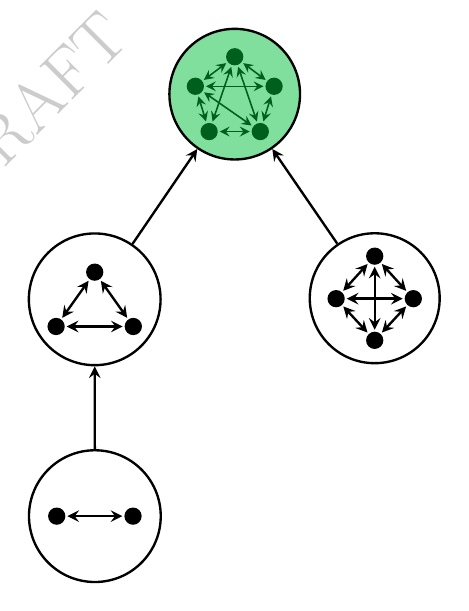
\begin{tikzpicture} %Anchored
\begin{scope}[scale=0.25]
\node(t)[circle,draw,inner sep=2pt,outer sep=1pt,line width=0.2mm,fill=black] at (0,2) {}; 
\node(ml)[circle,draw,inner sep=2pt,outer sep=1pt,line width=0.2mm,fill=black] at (-2,0.5){}; 
\node(mr)[circle,draw,inner sep=2pt,outer sep=1pt,line width=0.2mm,fill=black] at (2,0.5) {}; 
\node(bl)[circle,draw,inner sep=2pt,outer sep=1pt,line width=0.2mm,fill=black] at (-1.3,-1.8){}; 
\node(br)[circle,draw,inner sep=2pt,outer sep=1pt,line width=0.2mm,fill=black] at (1.3,-1.8){}; 

\path[stealth-stealth,draw,line width=0.2mm] (t)--(ml);
\path[stealth-stealth,draw,line width=0.2mm] (t)--(mr);
\path[stealth-stealth,draw,line width=0.2mm] (t)--(bl);
\path[stealth-stealth,draw,line width=0.2mm] (t)--(br);

\path[stealth-stealth,draw,line width=0.2mm] (ml)--(mr);
\path[stealth-stealth,draw,line width=0.2mm] (ml)--(br);
\path[stealth-stealth,draw,line width=0.2mm] (ml)--(bl);

\path[stealth-stealth,draw,line width=0.2mm] (mr)--(br);
\path[stealth-stealth,draw,line width=0.2mm] (bl)--(br);

\node[circle,fill=darkgreen, fill opacity = 0.5, draw=black,line width=0.3mm, fit=(t) (ml) (mr) (bl)(br), inner sep=-1pt] (r1) {};
\end{scope}


\begin{scope}[yshift=-0.8in,xshift=0.7in]
\node (t)[circle,draw,inner sep=2pt,outer sep=1pt,line width=0.2mm,fill=black] {}; 
\node (b)[circle,draw,inner sep=2pt,outer sep=1pt,line width=0.2mm,fill=black,below=0.8 of t] {}; 
\node(ml)[circle,draw,inner sep=2pt,outer sep=1pt,line width=0.2mm,fill=black,below left =0.35 and 0.3 of t]{}; 
\node(mr)[circle,draw,inner sep=2pt,outer sep=1pt,line width=0.2mm,fill=black,below right=0.35 and 0.3 of t]{}; 

\path[stealth-stealth,draw,line width=0.3mm] (t)--(ml);
\path[stealth-stealth,draw,line width=0.3mm] (t)--(mr);
\path[stealth-stealth,draw,line width=0.3mm] (ml)--(mr);
\path[stealth-stealth,draw,line width=0.3mm] (b)--(mr);
\path[stealth-stealth,draw,line width=0.3mm] (b)--(ml);
\path[stealth-stealth,draw,line width=0.3mm] (b)--(t);

\node[circle, draw=black,line width=0.3mm, fit=(t) (ml) (mr) (b), inner sep=-1.8pt] (r2) {};
\end{scope}

\begin{scope}[yshift=-0.88in,xshift=-0.7in]
\node (t)[circle,draw,inner sep=2pt,outer sep=1pt,line width=0.2mm,fill=black] {}; 
\node(ml)[circle,draw,inner sep=2pt,outer sep=1pt,line width=0.2mm,fill=black,below left =0.5 and 0.3 of t]{}; 
\node(mr)[circle,draw,inner sep=2pt,outer sep=1pt,line width=0.2mm,fill=black,below right=0.5 and 0.3 of t]{}; 

\path[stealth-stealth,draw,line width=0.3mm] (t)--(ml);
\path[stealth-stealth,draw,line width=0.3mm] (t)--(mr);
\path[stealth-stealth,draw,line width=0.3mm] (ml)--(mr);

\node[circle, draw=black,line width=0.3mm, fit=(t) (ml) (mr), inner sep=1pt] (r3) {};
\end{scope}

\begin{scope}[yshift=-2.1in,xshift=-0.89in]
\node(l)[circle,draw,inner sep=2pt,outer sep=1pt,line width=0.2mm,fill=black]{}; 
\node(r)[circle,draw,inner sep=2pt,outer sep=1pt,line width=0.2mm,fill=black,right=0.7 of l]{}; 

\path[stealth-stealth,draw,line width=0.3mm] (l)--(r);

\node[circle, draw=black,line width=0.3mm, fit=(l) (r), inner sep=4.7pt] (r4) {};
\end{scope}

\path[-stealth,draw,line width=0.3mm] (r2) -- (r1);
\path[-stealth,draw,line width=0.3mm] (r3) -- (r1);
\path[-stealth,draw,line width=0.3mm] (r4) -- (r3);

\end{tikzpicture}
}
\caption{A diagram of an anchored RPF with its mutually possible classes. The anchor class is shaded.}
\label{fig:anchored_rpf}
\end{figure}

\begin{figure}[h]
\centering
\resizebox{0.5\textwidth}{!}{
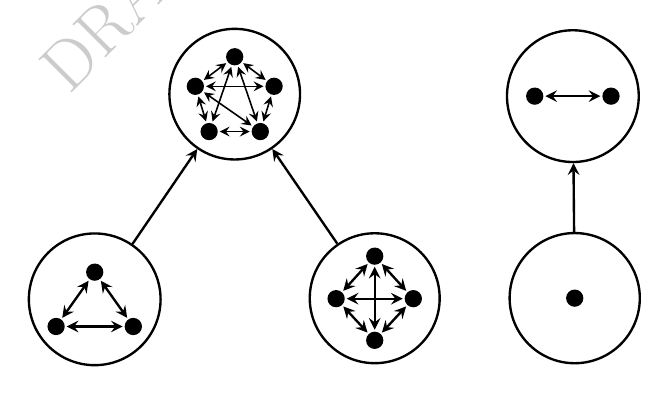
\begin{tikzpicture} %Non-Anchored
\begin{scope}[scale=0.25]
\node(t)[circle,draw,inner sep=2pt,outer sep=1pt,line width=0.2mm,fill=black] at (0,2) {}; 
\node(ml)[circle,draw,inner sep=2pt,outer sep=1pt,line width=0.2mm,fill=black] at (-2,0.5){}; 
\node(mr)[circle,draw,inner sep=2pt,outer sep=1pt,line width=0.2mm,fill=black] at (2,0.5) {}; 
\node(bl)[circle,draw,inner sep=2pt,outer sep=1pt,line width=0.2mm,fill=black] at (-1.3,-1.8){}; 
\node(br)[circle,draw,inner sep=2pt,outer sep=1pt,line width=0.2mm,fill=black] at (1.3,-1.8){}; 

\path[stealth-stealth,draw,line width=0.2mm] (t)--(ml);
\path[stealth-stealth,draw,line width=0.2mm] (t)--(mr);
\path[stealth-stealth,draw,line width=0.2mm] (t)--(bl);
\path[stealth-stealth,draw,line width=0.2mm] (t)--(br);

\path[stealth-stealth,draw,line width=0.2mm] (ml)--(mr);
\path[stealth-stealth,draw,line width=0.2mm] (ml)--(br);
\path[stealth-stealth,draw,line width=0.2mm] (ml)--(bl);

\path[stealth-stealth,draw,line width=0.2mm] (mr)--(br);
\path[stealth-stealth,draw,line width=0.2mm] (bl)--(br);

\node[circle, draw=black,line width=0.3mm, fit=(t) (ml) (mr) (bl)(br), inner sep=-1pt] (r1) {};
\end{scope}


\begin{scope}[yshift=-0.8in,xshift=0.7in]
\node (t)[circle,draw,inner sep=2pt,outer sep=1pt,line width=0.2mm,fill=black] {}; 
\node (b)[circle,draw,inner sep=2pt,outer sep=1pt,line width=0.2mm,fill=black,below=0.8 of t] {}; 
\node(ml)[circle,draw,inner sep=2pt,outer sep=1pt,line width=0.2mm,fill=black,below left =0.35 and 0.3 of t]{}; 
\node(mr)[circle,draw,inner sep=2pt,outer sep=1pt,line width=0.2mm,fill=black,below right=0.35 and 0.3 of t]{}; 

\path[stealth-stealth,draw,line width=0.3mm] (t)--(ml);
\path[stealth-stealth,draw,line width=0.3mm] (t)--(mr);
\path[stealth-stealth,draw,line width=0.3mm] (ml)--(mr);
\path[stealth-stealth,draw,line width=0.3mm] (b)--(mr);
\path[stealth-stealth,draw,line width=0.3mm] (b)--(ml);
\path[stealth-stealth,draw,line width=0.3mm] (b)--(t);

\node[circle, draw=black,line width=0.3mm, fit=(t) (ml) (mr) (b), inner sep=-1.8pt] (r2) {};
\end{scope}

\begin{scope}[yshift=-0.88in,xshift=-0.7in]
\node (t)[circle,draw,inner sep=2pt,outer sep=1pt,line width=0.2mm,fill=black] {}; 
\node(ml)[circle,draw,inner sep=2pt,outer sep=1pt,line width=0.2mm,fill=black,below left =0.5 and 0.3 of t]{}; 
\node(mr)[circle,draw,inner sep=2pt,outer sep=1pt,line width=0.2mm,fill=black,below right=0.5 and 0.3 of t]{}; 

\path[stealth-stealth,draw,line width=0.3mm] (t)--(ml);
\path[stealth-stealth,draw,line width=0.3mm] (t)--(mr);
\path[stealth-stealth,draw,line width=0.3mm] (ml)--(mr);

\node[circle, draw=black,line width=0.3mm, fit=(t) (ml) (mr), inner sep=1pt] (r3) {};
\end{scope}

\begin{scope}[xshift=1.5in]
\node(l)[circle,draw,inner sep=2pt,outer sep=1pt,line width=0.2mm,fill=black]{}; 
\node(r)[circle,draw,inner sep=2pt,outer sep=1pt,line width=0.2mm,fill=black,right=0.7 of l]{}; 

\path[stealth-stealth,draw,line width=0.3mm] (l)--(r);

\node[circle, draw=black,line width=0.3mm, fit=(l) (r), inner sep=4.7pt] (r4) {};
\end{scope}

\begin{scope}[yshift=-1.01in,xshift=1.7in]
\node(l)[circle,draw,inner sep=2pt,outer sep=1pt,line width=0.2mm,fill=black]{}; 

\node[circle, draw=black,line width=0.3mm, fit=(l), inner sep=12.8pt] (r5) {};
\end{scope}

\path[-stealth,draw,line width=0.3mm] (r2) -- (r1);
\path[-stealth,draw,line width=0.3mm] (r3) -- (r1);
\path[-stealth,draw,line width=0.3mm] (r5) -- (r4);
\end{tikzpicture}
}
\caption{This is the diagram for a single RPF that is not anchored. Notice that there is no anchored mutually possible class. This meams that we cannot turn this into an absolute probability function.}
\label{fig:unanchored_rpf} 
\end{figure}

Finally, we look at totally comparable RPFs, where the graph of mutually possible components is a straight line (see figure \ref{fig:totally_comparable_rpf}).

\begin{theorem}
If an RPF is totally comparable, then the equivalance classes of mutually possible outcomes are \textit{totally ordered}. That is, each member of an equivalence class of outcomes is comparable to each member of another class with that comparison always being 0 or \(\infty\).
\end{theorem}

\begin{proof}
Let A and B be 2 distinct mutually possible equivalence classes on \(\Omega\), and let \(a \in A\) and \(b \in B\). Then \(P(a, b)\) must be either 0 or \(\infty\) because if it were in between then \(a\) and \(b\) would be in the same equivalence class, and if it were \(\ast\) then \(P\) wouldn't be totally comparable.

Let \(a' \in A\) and \(b' \in B\). Then \(0 < P(a', a) < \infty\) and \(0 < P(b, b') < \infty\) due to the definition of mutual comparability. Thus with composition we get
\[P(a', b') :\cong P(a', a) \cdot P(a, b) \cdot P(b, b') = P(a, b)\]

Therefore, all comparisons between the 2 classes will be the same, and they will either be 0 or \(\infty\).
\end{proof}

\begin{figure}[h]
\centering
\resizebox{0.1\textwidth}{!}{
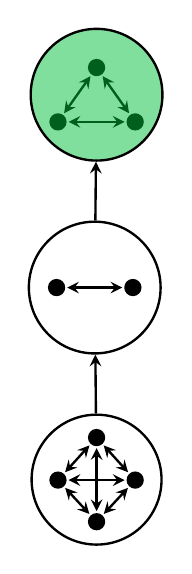
\begin{tikzpicture} %Totally Comparable
\begin{scope}
\node (t)[circle,draw,inner sep=2pt,outer sep=1pt,line width=0.2mm,fill=black] {}; 
\node(ml)[circle,draw,inner sep=2pt,outer sep=1pt,line width=0.2mm,fill=black,below left =0.5 and 0.3 of t]{}; 
\node(mr)[circle,draw,inner sep=2pt,outer sep=1pt,line width=0.2mm,fill=black,below right=0.5 and 0.3 of t]{}; 

\path[stealth-stealth,draw,line width=0.3mm] (t)--(ml);
\path[stealth-stealth,draw,line width=0.3mm] (t)--(mr);
\path[stealth-stealth,draw,line width=0.3mm] (ml)--(mr);

\node[circle, fill=darkgreen, fill opacity = 0.5, draw=black,line width=0.3mm, fit=(t) (ml) (mr), inner sep=1pt] (r1) {};
\end{scope}

\begin{scope}[yshift=-1.1in,xshift=-0.2in]
\node(l)[circle,draw,inner sep=2pt,outer sep=1pt,line width=0.2mm,fill=black]{}; 
\node(r)[circle,draw,inner sep=2pt,outer sep=1pt,line width=0.2mm,fill=black,right=0.7 of l]{}; 

\path[stealth-stealth,draw,line width=0.3mm] (l)--(r);

\node[circle, draw=black,line width=0.3mm, fit=(l) (r), inner sep=4.7pt] (r2) {};
\end{scope}

\begin{scope}[yshift=-1.85in]
\node (t)[circle,draw,inner sep=2pt,outer sep=1pt,line width=0.2mm,fill=black] {}; 
\node (b)[circle,draw,inner sep=2pt,outer sep=1pt,line width=0.2mm,fill=black,below=0.8 of t] {}; 
\node(ml)[circle,draw,inner sep=2pt,outer sep=1pt,line width=0.2mm,fill=black,below left =0.35 and 0.3 of t]{}; 
\node(mr)[circle,draw,inner sep=2pt,outer sep=1pt,line width=0.2mm,fill=black,below right=0.35 and 0.3 of t]{}; 

\path[stealth-stealth,draw,line width=0.3mm] (t)--(ml);
\path[stealth-stealth,draw,line width=0.3mm] (t)--(mr);
\path[stealth-stealth,draw,line width=0.3mm] (ml)--(mr);
\path[stealth-stealth,draw,line width=0.3mm] (b)--(mr);
\path[stealth-stealth,draw,line width=0.3mm] (b)--(ml);
\path[stealth-stealth,draw,line width=0.3mm] (b)--(t);

\node[circle, draw=black,line width=0.3mm, fit=(t) (ml) (mr) (b), inner sep=-1.8pt] (r3) {};
\end{scope}

\path[-stealth,draw,line width=0.3mm] (r2) -- (r1);
\path[-stealth,draw,line width=0.3mm] (r3) -- (r2);
\end{tikzpicture}
}
\caption{This is a diagram of a totally comparable RPF that is not mutually possible. The mutually possible components form a total order, with the \textit{anchored component} - which contains all anchor elements - is on top.}
\label{fig:totally_comparable_rpf}
\end{figure}

\subsection{Totally Mutually Possible RPFs}

\begin{definition}
\label{def:totally_mutually_possible}
A relative probability function is called \textit{totally mutually possible} if all of its outcomes\footnote{Note that this one of the few definitions that cannot be upgraded from outcomes to events. The empty event \(e = \{\}\) for example will be impossible with respect to any outcome by theorem \ref{thm:empty_event_impossible}.} are mutually possible. Mutually possible RPFs satisfy \textit{Cromwell's rule} in Bayesian inference, which states that prior beliefs should not assign probability zero or one to events\footnote{It would be stated differently in continuous space.}.
\end{definition}

Totally mutually possible RPFs have a simple diagram where all the outcomes are completely connected as in figure \ref{fig:mutually_possible_rpf}. All of the outcome are anchor outcomes, and there is a single mutually possible class.

\begin{figure}[]
\centering
\resizebox{0.2\textwidth}{!}{
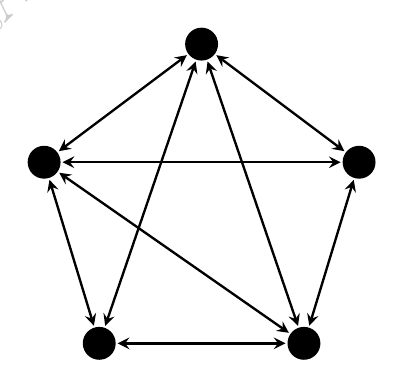
\begin{tikzpicture} %Totally Possible
\node(t)[circle,draw,inner sep=4pt,outer sep=1pt,line width=0.2mm,fill=black] at (0,2) {}; 
\node(ml)[circle,draw,inner sep=4pt,outer sep=1pt,line width=0.2mm,fill=black] at (-2,0.5){}; 
\node(mr)[circle,draw,inner sep=4pt,outer sep=1pt,line width=0.2mm,fill=black] at (2,0.5) {}; 
\node(bl)[circle,draw,inner sep=4pt,outer sep=1pt,line width=0.2mm,fill=black] at (-1.3,-1.8){}; 
\node(br)[circle,draw,inner sep=4pt,outer sep=1pt,line width=0.2mm,fill=black] at (1.3,-1.8){}; 

\path[stealth-stealth,draw,line width=0.3mm] (t)--(ml);
\path[stealth-stealth,draw,line width=0.3mm] (t)--(mr);
\path[stealth-stealth,draw,line width=0.3mm] (t)--(bl);
\path[stealth-stealth,draw,line width=0.3mm] (t)--(br);

\path[stealth-stealth,draw,line width=0.3mm] (ml)--(mr);
\path[stealth-stealth,draw,line width=0.3mm] (ml)--(br);
\path[stealth-stealth,draw,line width=0.3mm] (ml)--(bl);

\path[stealth-stealth,draw,line width=0.3mm] (mr)--(br);
\path[stealth-stealth,draw,line width=0.3mm] (bl)--(br);

\end{tikzpicture}
}
\caption{A totally mutually possible RFP has - unsurprisingly - a complete graph of mutually possibility.}
\label{fig:mutually_possible_rpf}
\end{figure}

\begin{theorem}
A non-empty totally mutually possible RPF is equal to an absolute probability function.
\end{theorem}

\begin{proof}
If \(P\) is non-empty, and totally mutually possible, all of it's outcomes are anchors. Therefore, we can use theorem \ref{thm:absolute_prob_formula} to find a matching absolute probability function
\[P(h) = \frac{P(h, a)}{\sum_{h' \in \Omega}P(h', a)}\]

Because every element of \(\Omega\) is an anchor, we can let \(a = h\) and get
\[P(h) = \frac{P(h, h)}{\sum_{h' \in \Omega}P(h', h)}=\frac{1}{\sum_{h' \in \Omega}P(h', h)}\]

Theorem \ref{thm:absolute_prob_formula} states that \(P(h_1, h_2) :\cong \frac{P(h_1)}{P(h_2}\), but since the constraint is never \(\ast\), they must be equal.
\end{proof}

We have thus constructed an RPF from its absoulte probability function without loss of information.

\section{From Outcomes to Events}

Our next task is to upgrade \(P\) to operate on the event level. This is more difficult than it seems. For example, we may wish to declare that the probability of event \(e_1\) with respect to \(e_2\) is going to be additive on \(e_1\) as follows:
\begin{equation}
\label{eq:incorrect_additive_event_def}
P(e_1, e_2) = \sum_{h_1 \in e_1}P(h_1, e_2)
\end{equation}

Equation \ref{eq:incorrect_additive_event_def} looks uncontroversial, but it actually contradicts the fundamental axioms! If we let \(e_1 = \varnothing\), then we have an empty sum on the right hand side of the equation, and we get \(P(\varnothing, e_2) = 0\). Likewise, if we allow \(e_2\) to be empty, we get \(P(e_1, \varnothing) = P(\varnothing, e_1)^{-1}=0^{-1}=\infty\). Both of these statements make sense until you realize that \(P(\varnothing, \varnothing) = 0 = \infty\), and what's worse is that they are also equal 1 under the identity axiom!

Another problem arises when events are \textit{internally non-comparable}, meaning that event \(e\) contains outcomes \(h_1\) and \(h_2\) where \(P(h_1, h_2) = \ast\). Perhaps there are still a few interesting things we can say about such an event, but here we will constrain ourselves entirely to totally comparable outcome spaces in order to avoid such questions.

\begin{definition}
Let \(P\) be a totally comparable finite RPF. \(P\) can also measure the probability of two events relative to each other using the following rules:

\begin{enumerate}[(i)]
  \item \label{event_def_1} \(P(e_1, e_2)\) obeys the fundamental axioms of relative probability.
  \item \label{event_def_2} \(P(e_1, e_2)\) sums over any reference outcome \(h\), so long as the result isn't indeterminate.
    \begin{equation}
      \label{eq:event_def_ratio_match}
      P(e_1, e_2) :\cong \frac{\sum_{h_1 \in e_1} P(h_1, h)}{\sum_{h_2 \in e_2} P(h_2, h)}
    \end{equation}
\end{enumerate}
\end{definition}

Because we no longer have access to absolute probability, the best we can do is measure it relative to a \textit{reference outcome} \(h^*\). This ratio might be indeterminate, so we use the matching relation instead of equality. Fortunately, we can show that there exists at least one reference outcome that will constrain \(P(e_1, e_2\) in \ref{eq:event_def_ratio_match} if they are non-empty.

\begin{proof}
Each event in a totally comparable RPF must have an anchor internally, using the same argument made for proving the existance of anchors in lemma \ref{lemma:totally_comp_anchored}. Choose an internal anchor \(a\) from one of the events, say \(e_1\). Then the sum \(\sum_{h_1 \in e_1} P(h_1, a)\) will be non-infinite by definition of anchors, and non-zero because \(P(a, a) = 1\) is a term in the sum. Therefore, the constraint as a whole cannot be indeterminate.

If both events are empty, then we are unable to create an anchor element, but by the identity axiom \(P(\varnothing, \varnothing) = 1\).
\end{proof}

These requirements again seem reasonable, but how can we know for sure that they provide a complete and consistent definition of \(P: \mathcal{F} \times \mathcal{F} \rightarrow \mathbb{M}^*\)? The following must be shown:

\begin{enumerate}[(i)]
  \item \label{event_def_proof_1} If two distinct values for \(h^*\) in statement \ref{eq:event_def_ratio_match} yield constraints on \(P\), then they must be equal.
  \item \label{event_def_proof_2} The constraint in \ref{eq:event_def_ratio_match} will not violate the fundamental axioms.
\end{enumerate}

\begin{proof}
For \ref{event_def_proof_1}:

Let \(r_1\) and \(r_2\) be distinct reference outcomes, and both constrain \(P(e_1, e_2)\). Then we want to check that

\begin{equation}
\label{eq:relative_event_unique}
\frac{\sum_{h_1 \in e_1} P(h_1, r_1)}{\sum_{h_2 \in e_2} P(h_2, r_1)} = \frac{\sum_{h_1 \in e_1} P(h_1, r_2)}{\sum_{h_2 \in e_2} P(h_2, r_2)}
\end{equation}

Neither expression is a wildcard, and none of the individual terms are either. The key to this argument is in looking at the value of \(P(r_1, r_2)\).

Assume \(P(r_1, r_2) = 0\). 

Then if \(\sum_{h_1 \in e_1} P(h_1, r_1)\) is not infinite, then \(\sum_{h_1 \in e_1} P(h_1, r_2)\) must be zero. The same argument applies to \(\sum_{h_2 \in e_2} P(h_2, r_2)\). Since they can't both be zero, we can say that one of the sums on the left hand side is infinite, so that \(P(e_1, e_2)\) is either \(\infty\) or 0. Let's say it is 0. Then \(\sum_{h_1 \in e_1} P(h_1, r_1) = 0\) and \(\sum_{h_2 \in e_2} P(h_2, r_1) = \infty\) and by the argument above \(\sum_{h_1 \in e_1} P(h_1, r_2) = 0\). Because the right hand side is not \(\ast\) - it must resolve to zero as well. The same agument holds for \(P(e_1, e_2) = \infty\).

By an analogous argument, if \(P(r_1, r_2) \infty\) then equation \ref{eq:relative_event_unique} must hold.

So now we can assume that \(P(r_1, r_2) \notin {0, \infty} \). The allows us to multiply the left hand side of equation \ref{eq:relative_event_unique} by \(1 = \frac{P(r_1, r_2)}{P(r_1, r_2)}\) and distribute into the sum to get:

\[\frac{\sum_{h_1 \in e_1} P(h_1, r_1) \cdot P(r_1, r_2)}{\sum_{h_2 \in e_2} P(h_2, r_1) \cdot P(r_1, r_2)} = \frac{\sum_{h_1 \in e_1} P(h_1, h_2^*)}{\sum_{h_2 \in e_2} P(h_2, h_2^*)}\]

For \ref{event_def_proof_2}:

The identity, inverse, and composition axioms easily follow from the fact that equation \ref{eq:event_def_ratio_match} is a ratio with identical terms for \(e_1\) in the numerator and \(e_2\) in the denominator. Therefore, if it resolves it is just a ratio of positive numbers - which can be shown to follow the 3 axioms.
\end{proof}

\begin{theorem}
Given events \(e_1\) and \(e_2\) where they are not both empty, we have \[P(e_1, e_2) = \sum_{h_1 \in e_1} \frac{1}{\sum_{h_2 \in e_2} P(h_2, h_1)}.\]
\end{theorem}

\begin{proof}
Start with the equation and multiply and use a suitable reference outcome \(h\).
\[\sum_{h_1 \in e_1} \frac{1}{\sum_{h_2 \in e_2} p(h_2, h_1)} :\cong \sum_{h_1 \in e_1} \frac{P(h_1, h)}{\sum_{h_2 \in e_2} P(h_2, h_1) P(h_1, h)} = \frac{\sum_{h_1 \in e_1} P(h_1, h)}{\sum_{h_2 \in e_2} P(h_2, h)}\]

Since both \(P(e_1, e_2)\) and the formula above match the same thing which is not always \(\ast\), they must be equal.
\end{proof}

We then derive the absolute probability function as
\[P(e) = P(e, \Omega) = \sum_{h \in e} \frac{1}{\sum_{h' \in \Omega}p(h', h)}\]

\begin{theorem}
\label{thm:empty_event_impossible}
The empty event \(\varnothing\) has probability 0 with respect to any non-empty event.
\end{theorem}

\begin{proof}
Let \(e\) be a non-empty event, and let \(h\) be an outcome in \(e\).

\[P(\varnothing, e) :\cong \frac{\sum_{h_1 \in \varnothing} P(h_1, h)}{\sum_{h_2 \in e} P(h_2, h)} = \frac{0}{\sum_{h_2 \in e} P(h_2, h)}\]

The denominator cannot itself be zero because \(P(h, h)\) is one of the terms. Therefore, \(P(\varnothing, e) = 0\)
\end{proof}

\section{Composing Relative Probability Functions}

Let \(P_0, P_1, ..., P_{K-1}\) be relative probability functions. Each of these probability functions have unique categories in their own right.

Let the set of outcomes acted upon by \(P_k\) be \(\Omega_k\), so that \(P_k: \Omega_k \times \Omega_k \rightarrow \mathbb{M}^{\ast}\). We take all \(\Omega_k\) to be disjoint from one another.

We can combine all of these relative probability functions together with a top level probability function \(P_\top\)\footnote{Pronounced \quotes{P-Top}.} with outcome space \(\Omega_\top = \{\Omega_0, \Omega_1, \Omega_2, ... \Omega_{K- 1}\}\).

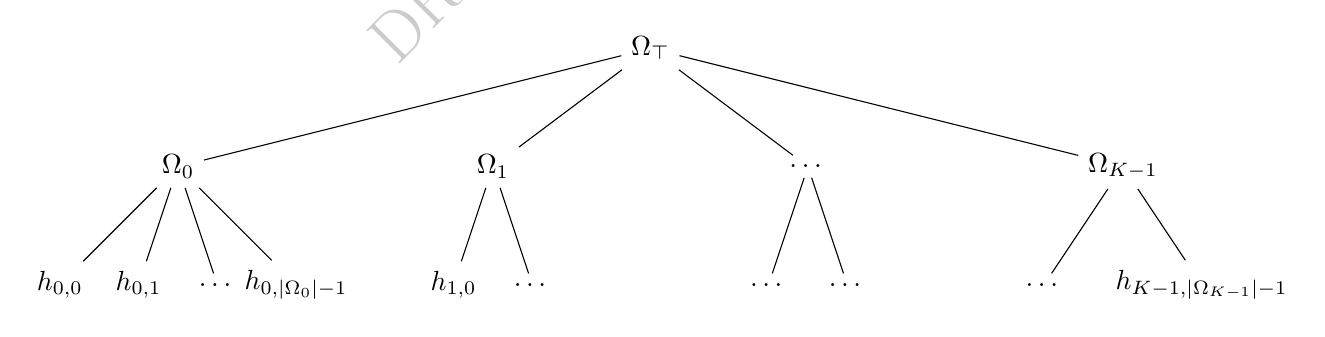
\begin{tikzpicture}
\node {\(\Omega_\top\)} [sibling distance = 4cm]
  child {node {\(\Omega_0\)}  [sibling distance = 1cm]
    child {node {\(h_{0, 0}\)}}
    child {node {\(h_{0, 1}\)}}
    child {node {\dots}}
    child {node {\(h_{0, |\Omega_0| - 1}\)}}
  }
  child {node {\(\Omega_1\)}  [sibling distance = 1cm]
    child {node {\(h_{1, 0}\)}}
    child {node {\dots}}  
  }
  child {node {\dots}  [sibling distance = 1cm]
    child {node {\dots}}
    child {node {\dots}}
  }
  child {node {\(\Omega_{K-1}\)}   [sibling distance = 2cm]
    child {node {\dots}}
    child {node {\(h_{K-1, |\Omega_{K-1}| - 1}\)}}
  };
\end{tikzpicture}

Now let \(\Omega\) be the set of all outcomes \(\Omega_0 \cup \Omega_1 \cup \dots \Omega_{K-1}\). We can create a new RPF - just called \(P\) acting on \(\Omega\) - with the following assumptions:

1) If the two outcomes fall under the same component, then their relative probabilities do not change:

\begin{equation}
\label{rpf_composition_same_branch}
P(h_{k, i}, h_{k, j}) = P_k(h_{k, i}, h_{k, j})
\end{equation}

2) If the two outcomes fall under different components, then their relative probabilities are given as follows.

\begin{equation}
\label{eq:rpf_composition_different_branch}
P(h_{k_1, i}, h_{k_2, j}) = P_{k_1}(h_{k_1, i}, \Omega_{k_1}) \cdot  P_{\top}(\Omega_{k_1}, \Omega_{k_2}) \cdot P_{k_2}(\Omega_{k_2}, h_{k_2, j})
\end{equation}

Note the use of the composition property to traverse up and down the tree. One could of course imagine this for a tree being many levels, and having a different height for each branch.

\begin{theorem}
\(P\) respects the fundamental axioms.
\end{theorem}

\begin{proof}
Identity is obvious because an outcome is on the same component as itself, so we can use equation \ref{rpf_composition_same_branch} to get \(P(h_{k, i}, h_{k, i}) = P_k(h_{k, i}, h_{k, i}) = 1\)

The inverse and composition laws must be true if both inputs are in the same component, because that component already follows the axioms. We now look at two inputs are from different components.

The inverse law can be proven by calculation.
\begin{equation}
\begin{aligned}
P(h_{k_1, i}, h_{k_2, j})^{-1} &= (P_{k_1}(h_{k_1, i}, \Omega_{k_1}) \cdot  P_{\top}(\Omega_{k_1}, \Omega_{k_2}) \cdot P_{k_2}(\Omega_{k_2}, h_{k_2, j}))^{-1} \\
& = P_{k_1}(h_{k_1, i}, \Omega_{k_1})^{-1} \cdot  P_{\top}(\Omega_{k_1}, \Omega_{k_2})^{-1} \cdot P_{k_2}(\Omega_{k_2}, h_{k_2, j})^{-1} \\
& = P_{k_1}(\Omega_{k_1}, h_{k_1, i}) \cdot  P_{\top}(\Omega_{k_2}, \Omega_{k_1}) \cdot P_{k_2}(h_{k_2, j}, \Omega_{k_2}) \\
& = P_{k_2}(h_{k_2, j}, \Omega_{k_2})\cdot  P_{\top}(\Omega_{k_2}, \Omega_{k_1}) \cdot P_{k_1}(\Omega_{k_1}, h_{k_1, i}) \\
& = P(h_{k_2, j}, h_{k_1, i})
\end{aligned}
\end{equation}

Composition can be shown similarly - now naming the 3 separate indecies in components \(k_1, k_2, k_3\) as \(i_1, i_2, i_3\) respectively.
\begin{equation}
\begin{aligned}
& P(h_{k_1, i_1}, h_{k_2, i_2}) \cdot P(h_{k_2, i_2}, h_{k_3, i_3}) \\
& :\cong P_{k_1}(h_{k_1, i_1}, \Omega_{k_1}) \cdot  P_{\top}(\Omega_{k_1}, \Omega_{k_2}) \cdot \textcolor{red}{P_{k_2}(\Omega_{k_2}, h_{k_2, i_2}) \cdot  P_{k_2}(h_{k_2, i_2}, \Omega_{k_2})} \cdot  P_{\top}(\Omega_{k_2}, \Omega_{k_3}) \cdot P_{k_3}(\Omega_{k_3}, h_{k_3, i_3}) \\
& :\cong P_{k_1}(h_{k_1, i_1}, \Omega_{k_1}) \cdot  \textcolor{red}{P_{\top}(\Omega_{k_1}, \Omega_{k_2}) \cdot  P_{\top}(\Omega_{k_2}, \Omega_{k_3})} \cdot P_{k_3}(\Omega_{k_3}, h_{k_3, i_3}) \\
& :\cong P_{k_1}(h_{k_1, i_1}, \Omega_{k_1}) \cdot  P_{\top}(\Omega_{k_1}, \Omega_{k_3}) \cdot P_{k_3}(\Omega_{k_3}, h_{k_3, i_3}) \\
& :\cong P_{k_1}(h_{k_1, i_1}, h_{k_3, i_3})
\end{aligned}
\end{equation}
\end{proof}

\begin{theorem}
\(P\) is totally comparable if and only if the following are true:

\begin{enumerate}
\item \(P_{\top}\) is totally comparable.
\item For all \(k \in \{0, 1, ..., K - 1\}\), \(P_k\) is totally comparable.
\item All components except at most one are totally mutually possible.
\item If there is a component that is not totally mutually possible, then every element of \(P_{\top}\) possible with respect to that component.
\end{enumerate}
\end{theorem}

\begin{proof}
If all the components are totally comparable, then we only need to prove that outcomes in different components are comparable. Starting with equation \ref{eq:rpf_composition_different_branch},

\begin{equation}
P(h_{k_1, i}, h_{k_2, j}) = P_{k_1}(h_{k_1, i}, \Omega_{k_1}) \cdot  P_{\top}(\Omega_{k_1}, \Omega_{k_2}) \cdot P_{k_2}(\Omega_{k_2}, h_{k_2, j})
\end{equation}

The only way that we can get \(P(h_{k_1, i}, h_{k_2, j}) = \ast\) is if there are both \(0\) and \(\infty\) as factors on the right hand side.

Because there is at most one component with outcomes impossible with respect to that component, we can say that either \(P_{k_1}(h_{k_1, i}, \Omega_{k_1}) = 0\) or \(P_{k_2}(h_{k_2, j}, \Omega_{k_2}) = 0\), or possibly neither, but not both.

Neither can be infinite either by the definition of the event level in equation \ref{eq:event_def_ratio_match}. Here we look at the factor \(P_{k_1}(h_{k_1, i}\) and use \(k_1\) itself as the reference outcome.
\[
P_{k_1}(h_{k_1, i}, \Omega_{k_1}) :\cong \frac{\sum_{h_1 \in \{k_1\}} P(h_1, k_1)}{\sum_{h \in \Omega_{k_1}} P(h_2, k_1)} = \frac{1}{\sum_{h \in \Omega_{k_1}} P(h_2, k_1)}
\]

The denominator cannot be zero since \(P(k_1, k_1) = 1\) will be one of the terms under the sum.

If the \(P_{k_1}(h_{k_1, i} = 0\), then the only way the entire right hand side can be \(\ast\) is if \(P_{\top}(\Omega_{k_1}, \Omega_{k_2}) = \infty\). But this can't be true because we assumed that \(\Omega_{k_2}\) is possible with respect to \(\Omega_{k_1}\), the sole component with impossible outcomes!

An analogous argument can be made if \(P_{k_2}(h_{k_2, j}, \Omega_{k_2} = 0\).

Therefore, the right hand side of the equation is not \(\ast\) and \(P\) is totally comparable.

In the opposite direction, we can show that if any of the conditions are broken, then \(P\) is not totally comparable. Breaking any of the first two conditions would introduce an explicit \(\ast\) into equation \ref{eq:rpf_composition_different_branch}. If there are multiple components with impossible outcomes, then it would introduce a \(0\) into the first term of equation \ref{eq:rpf_composition_different_branch} and an \(\infty\) into the third term, yielding \(\ast\).

And finally, if only the fourth condition is broken, it would introduct a 0 into the first term of equation \ref{eq:rpf_composition_different_branch} and an \(\infty\) into the \textbf{second} term of equation \ref{eq:rpf_composition_different_branch}.

Therefore, if any of these conditions are broken, \(P\) is \textbf{not} totally comparable.
\end{proof}

\section{Bayesian Inference on Relative Distributions}

A relative probability function represents a belief over the set of potential hypotheses in \(\Omega\).

Start with the Bayesian inference formula for conditional probability for \(h \in \Omega\) assuming that we recieve data \(D\).

\[P(h|D) = \frac{P(D|h) \cdot P(h)}{P(D)} \qquad P(D) = \sum_{h \in \Omega} P(D|h) \cdot P(h)\]

Now we convert to relative probability by looking at the ratio between the two hypotheses.

\[\frac{P(h_1|D)}{P(h_2| D)} = \frac{P(D|h_1) \cdot P(h_1)}{P(D)} \div \frac{P(D|h_2) \cdot P(h_2)}{P(D)} = \frac{P(D|h_1) \cdot P(h_1)}{P(D|h_2) \cdot P(h_2)} \]

Notice that each component is represented by a ratio. By making the appropriate subsitutions, we can express this entirely in terms of relative probability functions.

For the ratio of prior probabilities, substitute the relative prior: \(\frac{P(h_1)}{P(h_2)} \rightarrow P(h_1, h_2) \)

For the ratio of posterior probabilities, substitute the relative posterior: \(\frac{P(h_1|D)}{P(h_2|D)} \rightarrow P(h_1, h_2|D) \)

It is more difficult to see that the likelihood ratio is a relative probability, but the Kolmogorov definition to expand conditional probability suggests that it is:

\[\frac{P(D|h_1)}{P(D|h_2)} = \frac{\frac{P(D \cap h_1)}{P(D)}}{\frac{P(D \cap h_2)}{P(D)}} = \frac{P(D \cap h_1)}{P(D \cap h_2)} \]

Therefore, we can let \(P_D\) represent the likelihood ratio of the different hypotheses, and we can be sure that it fits the RPF framework with regards to the fundamental axioms. The likelihood ratio \(P_D(h_1, h_2)\) encodes a description of how the different hypotheses rate the likelihood of data.

The substitution for the liklihood ratio is as follows: \(\frac{P(D|h_1)}{P(D|h_2)} \rightarrow P_D(h_1, h_2) \)

Now we get bayes rule for relative probability:

 \[P(h_1, h_2|D) = P_D(h_1, h_2) P(h_1, h_2)\]
 
Bayesian inference is not reduced to an element-by-element multiplication of two different RPFs: \(P_D(h_1, h_2)\) and \(P(h_1, h_2)\). Fortunately, product of two RPFs also obeys the fundamental axioms.

\begin{theorem} 
Let \(P_1\) and \(P_2\) be relative probability functions on \(\Omega\). Define \(P(h_1, h_2) = P_1(h_1, h_2) \cdot P_2(h_1, h_2)\). Then, \(P\) is also an RPF, that it is obeys the fundamental axioms.
\end{theorem}

\begin{proof} 
Use the multiplication property of the matching relation in equation \ref{theorem:matching_multiplication}.
 
Identity: \[P(h_1, h_1) = P_1(h_1, h_1) P_2(h_1, h_1)=1 \cdot 1=1\]
 
Inverse: \[P(h_1, h_2) = P_1(h_1, h_2) \cdot P_2(h_1, h_2)=P_1(h_2, h_1)^{-1} \cdot P_2(h_2, h_1)^{-1}=(P_1(h_2, h_1) \cdot P_2(h_2, h_1))^{-1}=P(h_2, h_1)^{-1}\]
 
Composition: \[P(h_1, h_2)P(h_2, h_3)=P_1(h_1, h_2) P_2(h_1, h_2)P_1(h_2, h_3) P_2(h_2, h_3) :\cong P_1(h_1, h_3) P_2(h_1, h_3)=\]
\end{proof}

\begin{theorem}
Once two outcomes become uncomparable, they will never be comparable again. In other words, if \(P(h_1, h_2)=\ast\), then \(P(h_1, h_2|D) = \ast\).
\end{theorem}

\begin{proof}
\(P(h_1, h_2|D) = L(D|h_1, h_2) P(h_1, h_2) = P_D(h_1, h_2) \cdot \ast = \ast\)
\end{proof}

\begin{theorem}
Once an outcome becomes impossible with respect to another event, it will either remain impossible or become uncomparable. In other words,  if \(P(h_1, h_2)=0\), then \(P(h_1, h_2|D) \in {0, \ast}\).
\end{theorem}

\begin{proof}
\(P(h_1, h_2|D) = L(D|h_1, h_2) P(h_1, h_2) = P_D(h_1, h_2) \cdot 0\). Normally, this would simplify to 0, but with the matching relation in \(\mathbb{M}^*\), this will be \(\ast\) if \(P_D(h_1, h_2) \in {\infty, \ast}\).
\end{proof}

\subsection{Example: A Noisy Channel}

Here is an example of how relative probability gives us an interesting way of looking at inference problems.

Suppose we are to recieve a message in outcome space \(\Omega = \{0, 1, ..., K-1\}\). There is a probability of \(p\) that the message goes through correctly. Otherwise, it gets scrambled and we recieve a value in \(\Omega\) drawn from the uniform distribution\footnote{We could still have gotten lucky and recived the correct value in this case}. We recieve the same message several times for redundancy, and count \(c_i\) as the number of times the message was recieved as \(k\).

To start with absolute probability, we can use the indicator function to get the probability of recieving \(h_1\) given that the real message was \(h_2\) is \(p[h_1 = h_2] + \frac{1-p}{K}\). We then use this to construct an RPF for the liklihood ratio if we recieve a single message, \(k\).
\[P_k(h_1, h_2) = \frac{p[h_1 = k] + \frac{1-p}{K}}{p[h_2 = k] + \frac{1-p}{K}} = \frac{pK[h_1 = k] + 1-p}{pK[h_2 = k] + 1-p}\]

Now if we recieve multiple messages in the count vector \(c\):
\[P_c(h_1, h_2) = \prod_{k \in \Omega}\left(\frac{pK[h_1 = k] + 1-p}{pK[h_2 = k] + 1-p}\right)^{c_k}\]

Note that if \(k \notin \{h_1, h_2\}\) then the term for that k becomes \(\frac{1-p}{1-p} = 1\), so there are only terms that we care about. We will also assume \(h_1 \neq h_2\):
\begin{equation}
\begin{aligned}
P_c(h_1, h_2) &= \left(\frac{pK[h_1 = h_1] + 1-p}{pK[h_2 = h_1] + 1-p}\right)^{c_{h_1}} \left(\frac{pK[h_1 = h_2] + 1-p}{pK[h_2 = h_2] + 1-p}\right)^{c_{h_2}} \\
& = \left(\frac{pK + 1-p}{1-p}\right)^{c_{h_1}} \left(\frac{1-p}{pK + 1-p}\right)^{c_{h_2}} = \left(1 + \frac{pK}{1-p}\right)^{c_{h_1} - c_{h_2}}
\end{aligned}
\end{equation}

Because the prior is uniform, we also get the posterior:
\[P(h_1, h_2 | c) = P_c(h_1, h_2) \cdot P(h_1, h_2) = \left(1 + \frac{pK}{1-p}\right)^{c_{h_1} - c_{h_2}} \]

Note that the relative probability between two hypotheses is exponential on the difference between their counts. Formulating these problems in terms of relative probability often lead to easily interpretable results, even before converting into absolute probability (if that is even required). Using a different prior would be as easy as appending an additional term.

\section{Implementation}

Finally, we implement relative probabiliy as a python class as a demonstration of its usage and relevance.

How to implement this in code, and point to open source example.

Note the connection between magnitude space and the extended real number line, which we can implement through floating point numbers.

This can be implemented by storing K values.

For each category, we have a tier. Items in the same tier are comparable. Each Tier has a parent tier, where items in this teir are said to be impossible relative to anything in its ancestor tiers.

For each category, we also store a floating point number called the value, which should be taken as the log of an unnormalized probability. Note that we will not allow inf or NaN here.

Get the relative probability of 2 categories. Algorithm: If they are in the same tier, then subtract their values and take the exp. If they are in different tiers, do a graph search on the tier. If the first is < the second, the answer is 0. If the first is > the second, the answer is 1. And if they are uncomparable, then the answer is Wildcard, NaN.

Generate and indifferent distribution of category K. Algorithm: Create a single tier where all values are set to 0.

Change the relative probability of item \(k_1\) with respect to \(k_2\), and set it to \(q\). Algorithm: UNSURE

Set the probability \(k_1\) to some absolute value with respect to either the whole distribution, or to its tier.

Randomly sample from this distribution. Algorithm: Only look at the top tier.

Randomly sample from this distribution, but remove certain categories. Algorithm: If the top tier categories are gone, look to see if a top tier remains. If there are multiple top tiers, then there's no way to do it!

Ask: Is this distribution totally mutually possible? Algorithm: Look are a single top tier.

Ask: Is it totally comparable? Algorithm: Look for a linear list of tiers.

\section{Topology and Limits in Relative Probability Space}
\label{section:topology}

Mathematics can model the real world even through ideas that are theoretically impossible. For example, we might believe that a certain natural process cannot repeat an infinite number of times - that it just is not something allowed by the physical limitations of our universe. And even so, we might still take its value to be infinity in a model in order to get a bound on what that system will look like in \quotes{the long run}. One of the benefits of relative probability spaces is their properties with respect to limits. To this end, we prove here that when we take limits of totally comparable RPFs, the resulting RPF will also be totally comparable.

This effort caps off the most significant argument in favor of totally comparable RPFs. They hold their information under the operation of limits, while absolute probability does not.

There is some background in topology\footnote{See Mendelson (1990) \cite{mendelson} and Bradley et al. (2020) \cite{bradley} for texts with formal definitions and theorems.} required for this section.

\subsection{RPF Space and Compactness}

Because the set of absolute distributions for K is embedded in \(\mathbb{R}^K\), its topological properties are well understood. The simplex is closed, bounded, and compact. Practically, this means that any sequence of points on the simplex will converge to one or more points on the simplex allowing both pure and applied practicioners to talk about limit and boundary conditions.

This strategy fails for relative probabilities, because there is no obvious way to embed an RPF into euclidean space\footnote{Though it may be possible! See section \ref{section:euclidean_embedding}}. The relative probability space is more complicated, because at the corners of the simplex lurk entire subspaces where outcomes are still being compared in different ways!

\begin{definition}
\(\text{RPF}^{\ast}(K)\) is the set of relative probability functions of size K (where \(\Omega = \{0, 1, ..., K - 1\}\)). Likewise \(\text{RPF}(K)\) is the set of all totally comparable RPFs of size K.
\end{definition}

If the \(\text{RPF}(K)\) is compact, then information about the relative probabilites of events are preserved even as they approach zero relative to another event.

In order to prove compactness, we first must define a topology on \(\text{RPF}(K)\). This starts with finding a \textit{basis of open sets}.

The notion of an open set can change even if a topological space is restricted. For example, on the real number line \(\mathbb{R}\), we take the open interval (0, 1) as an open set (as the term open interval suggests). However, once this is embedded into \(\mathbb{R}^2\), it is now a line segment in a plane and no longer open (see figure \ref{fig:sub_topology}). It can be thought of as a restriction to an open set on \(\mathbb{R}^2\) to \(\mathbb{R}\). For example, the set \(\{(x, y): x \in (0, 1)\;  \text{and}\;  y \in (-\epsilon, +\epsilon)\}\) given an \(\epsilon > 0\) is such an open set on \(\mathbb{R}^2\).

\begin{figure}[h]
\centering
\resizebox{0.4\textwidth}{!}{
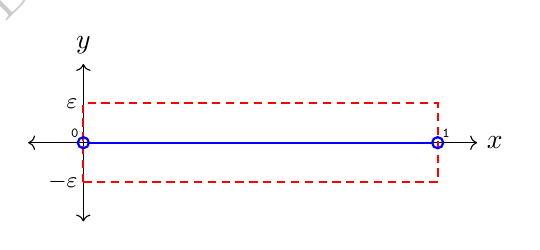
\begin{tikzpicture} %episilon diagram
\draw[<->] (-0.7,0)--(5,0) node[right] {\(x\)};
\draw[<->] (0,-1,0)--(0,1) node[above] {\(y\)};
\draw[densely dashed,red,thick] (0,-0.5) rectangle (4.5,0.5);
\draw[draw=blue,thick] (0,0) circle (2pt) node[above left=-0.1,font=\ttfamily\tiny] {0};
\draw[draw=blue,thick] (4.5,0) circle (2pt) node [above right=-0.1,font=\ttfamily\tiny] {1};

\node[left=-0.05,font=\ttfamily\footnotesize] at (0,-0.5) {\(-\varepsilon\)};
\node[left=-0.05,font=\ttfamily\footnotesize] at (0,0.5) {\(\varepsilon\)};
\node[circle,inner sep=1pt] at (0,0) (0){};
\node[circle,inner sep=1pt] at (4.5,0) (1){};
\path[draw,blue,thick] (0)--(1);
\end{tikzpicture}
}
\caption{The small box that is the interior of the dotted rectangle is an open set in \(\mathbb{R}^2\), and therefore its restriction to \(\mathbb{R}\) - the line segment - is an open set in \(\mathbb{R}\). But the line segment is not open in \(\mathbb{R}^2\).}
\label{fig:sub_topology}
\end{figure}


Likewise, an open set on a relative probability space restricted on several outcomes might not be an open set on the relative probability spaces for all of \(\Omega\).

We start by looking at RPFs with \(K = 2\). Fortunately, we find a totally comparable RPF that corresponds 1:1 with the magnitude space.

\begin{theorem}
Let \(\Omega = \{h_1, h_2\}\) have two elements, with relative probability function \(P\). Then, \(P\) is completely determined by \(P(h_1, h_2)\).
\end{theorem}

\begin{proof}
Let \(q = P(h_1, h_2)\). By the inverse symmetric property, \(P(h_2, h_1) = q^{-1}\). These values completely determine \(P\) on the outcome level.
\end{proof}

This gives us both a topology and a compactness proof for K = 2 for free because \(\text{RPF}(2)\) is isomorphic to \(\mathbb{M}\) which already has a natural topology. Its basis for open sets are the open intervals of \(\mathbb{B}\), including those intervals that include 0 and \(\infty\). For \(K > 2\), we will need more powerful tools.

\subsection{Open Patches}

We now develop a notion of open patches, which will be a basis of open sets on the space \(\text{RPF}(K)\).

\begin{definition}
An \textit{interior open patch} of \(\text{RPF}_{\text{comp}}(\Omega)\) is one of the following:

\begin{enumerate}
  \item If \(K = 2\), a subset parameterized by an interior open interval of magnitudes. \(\{P | a < P(h_1, h_2) < b\}\) for some \(a, b \in \mathbb{M}\) 
  \item If \(K > 2\), a composition of interor patches with composing function \(P_{\top}\) also being an interior patch.
\end{enumerate}
\end{definition}

Interior open patches contain only totally mutually possible functions. See figure \ref{fig:interior_open_patch}.

\begin{figure}[h]
\centering
\resizebox{0.4\textwidth}{!}{
\begin{tikzpicture}
\node {\(P_\top\)} [sibling distance = 3cm]
  child {node {\(P_0\)}  [sibling distance = 3cm]
    child {node {A}}
    child {node {B}}
  }
  child {node  {C}};
\end{tikzpicture}
}
 \hspace{3em}
\resizebox{0.4\textwidth}{!}{
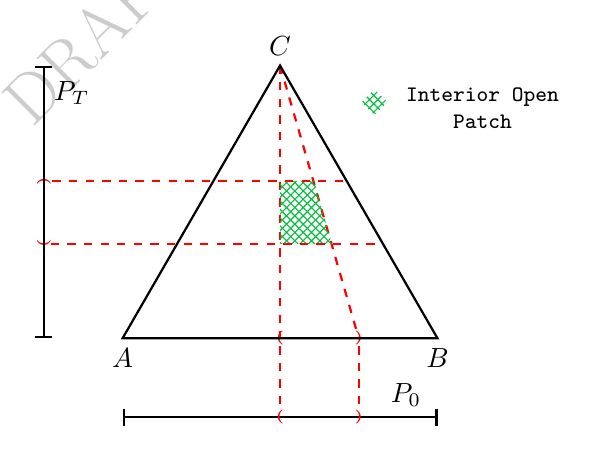
\begin{tikzpicture} %Triangle 3
\draw[thick, dashed,red] (0,{2*sqrt(3)})--(1,0) node [font=\tiny\bf] {)};
\draw[thick, dashed,red] (0,{2*sqrt(3)})--(0,0) node [font=\tiny\bf] {(};
\path[draw=none,pattern=crosshatch, pattern color=darkgreen] (0,1.2)--(0.66,1.2)--(0.43,2)--(0,2)--cycle;

\node[rectangle,rotate=45,draw=none,pattern=crosshatch, pattern color=darkgreen] at (1.2,3) (P){};

\node(Q)[rectangle,draw=none,align=center,below right=-0.3 and 0.1 of P,font=\ttfamily\footnotesize] {Interior Open\\ Patch};

\draw[thick] (-2,0)--(2,0)--(0,{2*sqrt(3)})--cycle;

\node (A) at (-2,0) [below] {\(A\)}; 
\node (B) at (2,0) [below] {\(B\)}; 
\node (C) at (0,{2*sqrt(3)}) [above] {\(C\)}; 

\draw[thick, dashed,red] (0.8,2)--(-3,2) node[font=\tiny\bf,rotate=90] {)};
\draw[thick, dashed,red] (1.2,1.2)--(-3,1.2) node[font=\tiny\bf,rotate=90] {(};

\draw[thick, dashed,red] (1,-0.1)--(1,-0.9);
\draw[thick, dashed,red] (0,-0.1)--(0,-0.9);

\draw[thick,|-|] (-3,0)--(-3,{2*sqrt(3)}) node[right,pos=0.9] {\(P_{T}\)};

\draw[thick,|-|] (-2,-1)--(2,-1) node[above,pos=0.9] {\(P_{0}\)} node[red,font=\tiny\bf] at (1,-1) {)}
node[red,font=\tiny\bf] at (0,-1) {(};
\end{tikzpicture}
}
\caption{An interior open patch captures a contiguous set inside the probability simplex. Above is an example of a composite probability distribution where the diagram on the left shows how \(P_\top\) and \(P_0\) are composed, and the right shows how the interior segments on both interact to form a patch. }
\label{fig:interior_open_patch}
\end{figure}

\begin{definition}
A \textit{facet\footnote{A facet of a simplex is a subset where one parameter is equal to zero - equivalent to a face on a 3D object.} patch} of \(\text{RPF}_{\text{comp}}(\Omega)\) is one of the following:

\begin{enumerate}
  \item If \(K = 2\), an interval of the form \(\{P | 0 < P(h_1, h_2) < a\}\) for some \(a \in \mathbb{M}\) 
  \item If \(K > 2\), the set of compositions where \(P_{\top}\) is drawn from an interior open patch, and all but one of the components are drawn from interior open patches. The last component - called the \textit{facet component} is itself a facet patch.
\end{enumerate}
\end{definition}

\begin{definition}
An \textit{exterior open patch} is a one of the following:

\begin{enumerate}
  \item Any facet patch.
  \item A composition where \(P_{\top}\) is a facet patch. The \textit{facet component} is itself drawn from any open patch, and all the other components are drawn from interior open patches.
\end{enumerate}
\end{definition}

Exterior open patches contain only totally mutually comparable functions, but some are not totally mutually possible. As seen in figure \ref{fig:exterior_open_patch}, they touch the hyperfaces (facets) of the simplex as well as the vertices and corners.  As the number of dimentions increase and the composition diagram changes, many more permutations are possible. Note that the point containing the corner at \(C\) is only half filled because the patch contains some values where \(P(C) = 1\) and not others, depending on the relative probability between \(A\) and \(B\).

\begin{figure}[h]
\centering
\resizebox{0.3\textwidth}{!}{
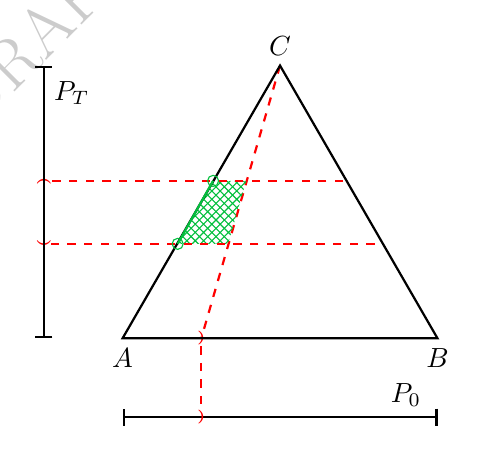
\begin{tikzpicture} %Triangle 2
\draw[thick, dashed,red] (0,{2*sqrt(3)})--(-1,0) node [font=\tiny\bf] {)};
\path[draw=none,pattern=crosshatch, pattern color=darkgreen] (-1.3,1.2)--(-0.66,1.2)--(-0.43,2)--(-0.86,2)--cycle;

\draw[thick] (-2,0)--(2,0)--(0,{2*sqrt(3)})--cycle;

\node (A) at (-2,0) [below] {\(A\)}; 
\node (B) at (2,0) [below] {\(B\)}; 
\node (C) at (0,{2*sqrt(3)}) [above] {\(C\)}; 

\draw[thick, dashed,red] (0.8,2)--(-3,2) node[font=\tiny\bf,rotate=90] {)};
\draw[thick, dashed,red] (1.2,1.2)--(-3,1.2) node[font=\tiny\bf,rotate=90] {(};

\draw[thick, dashed,red] (-1,-0.1)--(-1,-0.9);
\draw[thick, darkgreen] (-1.3,1.2)--(-0.85,2);

\draw[draw=darkgreen] (-1.3,1.2) circle (2pt);
\draw[draw=darkgreen] (-0.85,2) circle (2pt);

\draw[thick,|-|] (-3,0)--(-3,{2*sqrt(3)}) node[right,pos=0.9] {\(P_{T}\)};

\draw[thick,|-|] (-2,-1)--(2,-1) node[above,pos=0.9] {\(P_{0}\)} node[red,font=\tiny\bf] at (-1,-1) {)};
\end{tikzpicture}
}
\resizebox{0.3\textwidth}{!}{
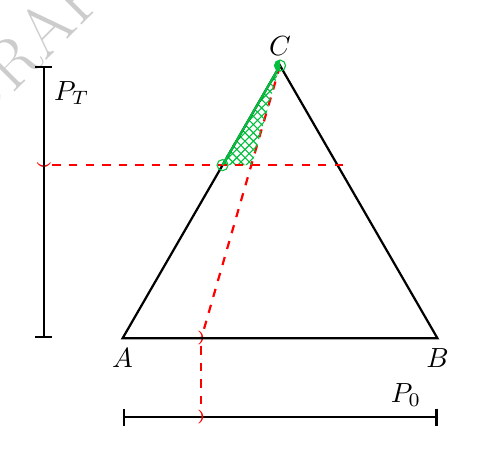
\begin{tikzpicture} %Triangle 1
\draw[thick, dashed,red] (0,{2*sqrt(3)})--(-1,0) node [font=\tiny\bf] {)};
\path[draw=none,pattern=crosshatch, pattern color=darkgreen] (-0.36,2.2)--(0,{2*sqrt(3)})--(-0.75,2.2)--cycle;

\draw[thick] (-2,0)--(2,0)--(0,{2*sqrt(3)})--cycle;

\node (A) at (-2,0) [below] {\(A\)}; 
\node (B) at (2,0) [below] {\(B\)}; 
\node (C) at (0,{2*sqrt(3)}) [above] {\(C\)}; 
\draw[thick, dashed,red] (0.8,2.2)--(-3,2.2) node[font=\tiny\bf,rotate=90] {(};
\draw[thick, dashed,red] (-1,-0.1)--(-1,-0.9);
\draw[thick, darkgreen] (-0.73,2.2)--(0,{2*sqrt(3)});

\draw[draw=darkgreen] (-0.73,2.2) circle (2pt);

\draw[draw=darkgreen] (0,{2*sqrt(3)}) circle (2pt);

\fill[darkgreen] (0,{2*sqrt(3)}) + (0, 2pt) arc (90:270:2pt);

\draw[thick,|-|] (-3,0)--(-3,{2*sqrt(3)}) node[right,pos=0.9] {\(P_{T}\)};

\draw[thick,|-|] (-2,-1)--(2,-1) node[above,pos=0.9] {\(P_{0}\)} node[red,font=\tiny\bf] at (-1,-1) {)};
\end{tikzpicture}
}
\resizebox{0.3\textwidth}{!}{
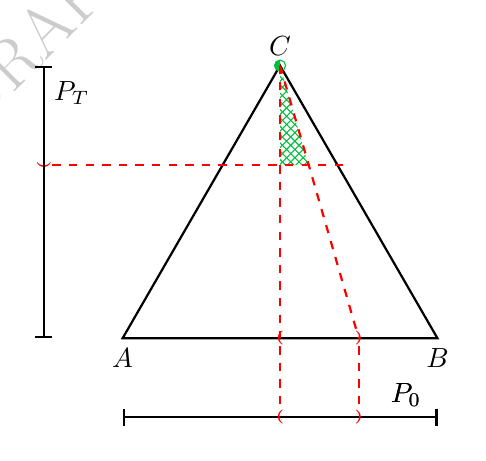
\begin{tikzpicture} %Triangle 1
\path[draw=none,pattern=crosshatch, pattern color=darkgreen] (0.36,2.2)--(0,{2*sqrt(3)})--(0,2.2)--cycle;

\draw[thick] (-2,0)--(2,0)--(0,{2*sqrt(3)})--cycle;

\node (A) at (-2,0) [below] {\(A\)}; 
\node (B) at (2,0) [below] {\(B\)}; 
\node (C) at (0,{2*sqrt(3)}) [above] {\(C\)}; 
\draw[thick, dashed,red] (0.8,2.2)--(-3,2.2) node[font=\tiny\bf,rotate=90] {(};

\draw[draw=darkgreen] (0,{2*sqrt(3)}) circle (2pt);

\fill[darkgreen] (0,{2*sqrt(3)}) + (0, 2pt) arc (90:270:2pt);

\draw[thick, dashed,red] (0,{2*sqrt(3)})--(1,0) node [font=\tiny\bf] {)};
\draw[thick, dashed,red] (0,{2*sqrt(3)})--(0,0) node [font=\tiny\bf] {(};

\draw[thick,|-|] (-3,0)--(-3,{2*sqrt(3)}) node[right,pos=0.9] {\(P_{T}\)};
\draw[thick,|-|] (-2,-1)--(2,-1) node[above,pos=0.9] {\(P_{0}\)};

\draw[thick, dashed,red] (1,-0.1)--(1,-0.9);
\draw[thick, dashed,red] (0,-0.1)--(0,-0.9);

\draw[thick,|-|] (-2,-1)--(2,-1) node[above,pos=0.9] {\(P_{0}\)}
node[red,font=\tiny\bf] at (1,-1) {)}
node[red,font=\tiny\bf] at (0,-1) {(};
\end{tikzpicture}
}
\caption{Examples of open patches. On the left is the facet patch, because it only touches a side (facet) of the simplex and not a corner. In the center is an exterior open patch where the facet component \(P_0\) is itself a facet patch (touching an edge and a corner), and on the right is an exterior open patch that touches a corner only because \(P_0\) is an interior open patch.}
\label{fig:exterior_open_patch}
\end{figure}

\begin{definition}
An \textit{open patch} is a subset of \(\text{RPF}(K)\) that is either an interior or exterior open patch.
\end{definition}

Now let the open patches be the bases for an open set thus defining a topology on \(\text{RPF}(K)\).

\begin{definition}
An \textit{open set} of \(\text{RPF}(K)\) is any (potentially infinite) union of open patches on \(\text{RPF}(K)\), or any finite intersection of open patches on \(\text{RPF}(K)\).
\end{definition}

\subsection{Compactness}

We will sketch out the compactness proof for \(\text{RPF}(K)\) here for brevity. First, we need a few lemmas.

\begin{lemma}
\label{lem:withhold_possible_outcome}
Let \(h\) be an outcome in \(\{0, 1, ..., K-1\}\), and let q be a number such that \(0 < q \leq 1\). The region of \(\text{RPF}(K)\) where the absolute probability of h is q is isomorphic to \(\text{RPF}(K-1)\).
\end{lemma}

\begin{proof}
If \(P(h) > 0\) then it is in the anchored equivalence class of mutually possibility. If \(P(h) = 1\) then the outcome \(h\) can be appended above any function in \(\text{RPF}(K - 1)\), and if \(P(h) < 1\) then \(h\) can be appended into the anchored equivalence class of any function in \(\text{RPF}(K-1)\). In both cases, a separate \(h\) with a given absolute probability can be appended to anything in \(\text{RPF}(K-1)\) to produce an element of \(\text{RPF}(K)\), with all elements of \(\text{RPF}(K)\) accounted for.
\end{proof}

\begin{lemma}
\label{lem:change_one_anchor_outcome}
Let \(h\) be an outcome in \(\{0, 1, ..., K-1\}\), and let \(P(h) > 0\). Given a number \(0 < q \leq 1\), there is a unique RPF \(P'\) which is equal to \(P\) when evaluated on outcomes \(\neq h\) and such that \(P'(h) = q\).
\end{lemma}

\begin{proof}
This will be a proof by construction. Let \(P'\) be the new distribution where \(h\) remains an anchor outcome, but its absolute probability has been changed to \(q\). For any anchor outcome \(a\), we set \(P'(a, h) = P(a, h) \cdot q \cdot P(a)^{-1} \)

For any non-anchor outcome \(b\), we note that \(P(b, h) = 0\) and therefore also \(P'(b, h) = 0\), otherwise \(b\) would now be possible relative to other anchors where it wasn't before.
\end{proof}

\begin{lemma}
\label{lem:open_anchor_outcome}
Let \(h\) be an outcome in \(\{0, 1, ..., K-1\}\), and let \(P(h) > 0\). Any open patch of \(\text{RPF}(K)\) that contains \(P\), also contains, for some open interval on \(\mathbb(M)\) containing \(P(h)\), all the values \(P'\) constructed through lemma \ref{lem:change_one_anchor_outcome} by setting \(P(h) = q\) for any \(q\) in that open interval.
\end{lemma}

\begin{proof}
\end{proof}

\begin{theorem}
\(\text{RPF}(K)\) is \textit{compact}, meaning that for every open cover of it, there is a finite subcover.
\end{theorem}

We will provide a sketch for the compactness proof here.

\begin{proof}
This is an inductive proof where we assume that the theorem is true for all \(k < K\) and then prove that it is true for \(K\).

If \(K \in {0, 1}\) then \(\text{RPF}(K)\) is finite and singular (either the empty RPF or unit RPF respectively). These are obviously compact. If \(K = 2\) then we have the topology of \(\mathbb{M}\) which is also compact (thanks to the \(\infty\) element).

Now we assume that \(K > 2\).

Consider the region of \(\text{RPF}(K)\) where a specific outcome is required to be the largest (or possibly ties for largest). In other words, for this special outcome \(h\), look at the region of \(\text{RPF}(K)\) where \(P(h', h) \leq  1\) for any other outcome \(h'\). There is one region for every outcome - \(K\)such regions overall - and collectively they cover \(\text{RPF}(K)\) but they are not disjoint. In fact, the uniform distribution belongs to all \(K\) regions!

If we can show that an open cover on \(\text{RPF}(K)\) has a finite subcover on a region, then it must have a finite subcover overall because there are a finite number of regions.

So consider one such region, and let \(h\) be the largest outcome from that region. \(h\) is an anchor element, which means that \(P(h, h') > 0\) for all \(h'\) when in fact it is \(\geq 1\). If \(P(h) = q\), then we know that \(\frac{1}{k} \leq q \leq 1\). By lemma \ref{lem:withhold_possible_outcome}, the rest of the distribution is isomorphic to \(\text{RPF}(K - 1)\) - and therefore compact by our inductive assumption. Therefore, there is a finite subcover covering all elements where \(P(h) = q\).

By lemma \ref{lem:open_anchor_outcome}, finite subcover will not just include cases where \(P(h) = q\), but will hold for some open interval around q as well.

So for each q where \(\frac{1}{K} \leq q \leq 1\), we have a finite subcover, with each subcover covering some open set around q. Because \([\frac{1}{K}, 1]\) is compact, all of these open sets around q have a finite subcover for the whole segment. This means that only finitely many of these q-based subcovers are required, and with each one being finite we have finitely many open sets for the entire region where \(h\) is the largest outcome.
\end{proof}

\section{Future Work}
\subsection{Expansions to infinite spaces}
The obvious extention is to expand relative probability to a generalized space which may be infinite, and thus capture all of the variety of probability distributions that one might wish to study and apply. This would start by modifying constaint \(eq:event_def_ratio_match\) to ask for an additive property on the level of families of infinite sets. The relative probability function would then become a \textit{relative probability distribution}.

This raises certain question which - while decisions have been made in prior work and certainly measure theory - should be open to discussion.
\begin{enumerate}
\item Do we need to keep countable additivity as set forth in the Kolmogorov axioms, or can we relax this to allow for a fair countable lottery? RPFs would provide a great way to analyze the fair countable lottery and this should be exploited!
\item If we derive a notion of probability density, then can these densities at a particular pair of events be used to compare the relative probability of those events? What specific properties of the relative probability distribution are required to make this work?
\end{enumerate}

It appears possible to use these ideas to create a unified version of the Hausdorff measure - which finds the size of an object given its dimention. Instead of considering it to be multiple measures - we can have a single measure where set can be compared to other sets of equal dimention, and smaller-dimentional objects are always mutually impossible to a larger dimentional objects.

\subsection{Relationship to Category Theory}

Category theorists will instantly recognize that an RPF describes a category perfectly. This construction can be analyzed and approached through the lens of category theory. Specifically, and RPF describes something called a \textit{thin category} where any pair of objects have at most one morphism connecting them (per direction).

\begin{center}
\resizebox{0.3\textwidth}{!}{
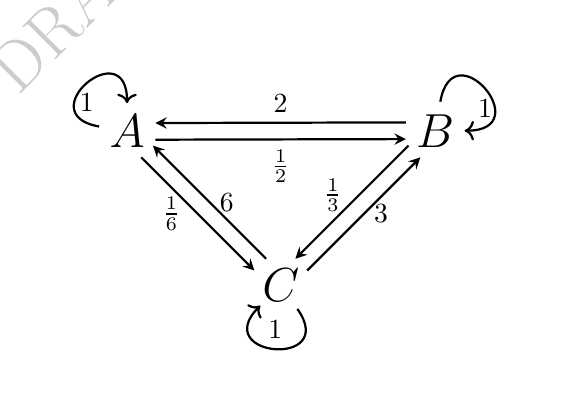
\begin{tikzpicture} %Commute Diagram
[node distance=0.8in]
\tikzset{
  shift left/.style ={commutative diagrams/shift left={#1}},
  shift right/.style={commutative diagrams/shift right={#1}},
  com/.style={circle,draw=none,inner sep=1pt,font=\LARGE}
}
\node (C) [com] {\(C\)};
\node (B) [com, above right = of C] {\(B\)};
\node (A) [com, above left = of C] {\(A\)};

\path[-stealth,thick,shift right=0.7ex] (C) edge node[right] {6} (A);
\path[-stealth,thick,shift right=0.7ex] (C) edge node[right] {3} (B);
\path[-stealth,thick,shift right=0.7ex] (B) edge node[above] {2} (A);


\path[-stealth,thick,shift right=0.7ex] (A) edge node[left,xshift=-0.6ex] {\(\frac{1}{6}\)} (C);
\path[-stealth,thick,shift right=0.7ex] (B) edge node[left,yshift=0.6ex] {\(\frac{1}{3}\)} (C);
\path[-stealth,thick,shift right=0.7ex] (A) edge node[below] {\(\frac{1}{2}\)} (B);

\path[<-,every loop/.style={looseness=5},thick] (A)
         edge  [in=170,out=90,loop,below] node {1} (); 
\path[<-,every loop/.style={looseness=5},thick] (B)
         edge  [in=80,out=0,loop,below] node {1} (); 
\path[<-,every loop/.style={looseness=9},thick,rotate=180] (C)
         edge  [in=-235,out=-315,loop,above] node {1} ();

%\path[-stealth,thick] (A) edge [loop above] node {1} ();
\end{tikzpicture}
}
\end{center}

The recent work of Censi et al.\cite{censi} concerns negative information in categories, ftwhich here corresponds to the wildcard element \(\ast\). It represents regions of the probability function that remain unassigned or uncomparable. This work could be used to subsume and further develop the idea of the indeterminate wildcard.

\subsection{Embedding in Euclidean Space}
\label{section:euclidean_embedding}

Absolute probability functions have this advantage where they can be embedded into a simplex in \(\mathbb{R}^K\). For relative probability functions, it is not so straightforward. However, it might be possible to derive a system for embedding RPFs into euclidean space. For example, the space \(\text{RPF}(3)\) can be mapped as a hexagon, where each point can be assigned a probability based on its distance between two parallel sides, which exist for each outcome.

\begin{center}[h]
\resizebox{0.25\textwidth}{!}{
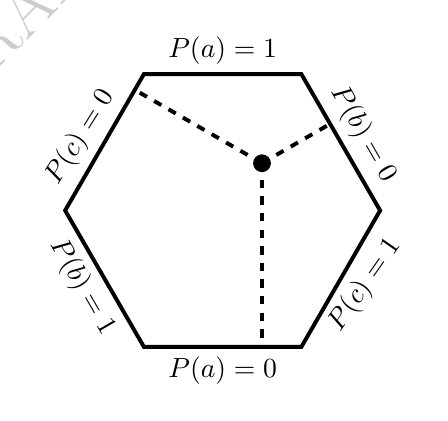
\begin{tikzpicture}
\node[regular polygon,draw,minimum size=4cm,line width=0.5mm,regular polygon sides = 6] (p) at (0,0) {};

\node at (p.corner 1) [anchor=360/6*(1-1)+270] {};
\node at (p.corner 2) [anchor=360/6*(2-1)+270] {};
\node at (p.corner 3) [anchor=360/6*(3-1)+270] {};
\node at (p.corner 4) [anchor=360/6*(4-1)+270] {};
\node at (p.corner 5) [anchor=360/6*(5-1)+270] {};
\node at (p.corner 6) [anchor=360/6*(6-1)+270] {};

\node[regular polygon,draw=none,rotate=30,minimum size=3.4cm,line width=0.5mm,regular polygon sides = 6] (A) at (0,0) {};
\node at (A.corner 1) [anchor=360/6*(1-1)+270] {\(P(a)=1\)};
\node at (A.corner 2) [anchor=360/6*(2-1)+230,rotate=58] {\(P(c)=0\)};
\node at (A.corner 3) [anchor=360/6*(4-1)+260,rotate=-60] {\(P(b)=1\)};
\node at (A.corner 4) [anchor=360/6*(4-1)+270] {\(P(a)=0\)};
\node at (A.corner 5) [anchor=360/6*(5-1)+230,rotate=55] {\(P(c)=1\)};
\node at (A.corner 6) [anchor=360/6*(7-1)+260,rotate=-60] {\(P(b)=0\)};

\draw[fill=black] (0.5,0.6) circle (3pt);

\draw[line width=0.5mm,dashed] (0.5,0.6) -- ($(p.corner 1)!(0.5,0.6)!(p.corner 6)$);
\draw[line width=0.5mm,dashed] (0.5,0.6) -- ($(p.corner 2)!(0.5,0.6)!(p.corner 3)$);
\draw[line width=0.5mm,dashed] (0.5,0.6) -- ($(p.corner 5)!(0.5,0.6)!(p.corner 4)$);
\end{tikzpicture}
}
\end{center}

In this case, the probability triangle has been truncated. For higher order simplcies, this appears to become exceedingly unweidly unless there is developed some simplifying trick. If it is successfully done, then the topological properties of \(\text{RPF}(K)\) fall into place easily.

It is also possible to hack a metric space for \(\text{RPF}(K)\) by assigning distances to elements based on their eucliean distance within their mutually possible class, and adding a corrective term depending on its location in the comparability graph. This may simplify the arguments in section \ref{section:topology}, and could potentially find use in algorithmic implementation.

%\subsubsection*{References}
\begin{thebibliography}{20}

\bibitem{sklar_dirichlet}Sklar, M. (2014). Fast MLE computation for the Dirichlet multinomial. arXiv preprint arXiv:1405.0099.
\bibitem{sklar_bias}Sklar, M. (2022). Sampling Bias Correction for Supervised Machine Learning: A Bayesian Inference Approach with Practical Applications. arXiv preprint arXiv:2203.06239.
\bibitem{mendelson}Mendelson, B. (1990). Introduction to topology. Courier Corporation.
\bibitem{bradley}Bradley, T. D., Bryson, T., \& Terilla, J. (2020). Topology: A Categorical Approach. MIT Press.
\bibitem{lyon}Lyon, A. (2016). Kolmogorov’s Axiomatisation and its Discontents. The Oxford handbook of probability and philosophy, 155-166.
\bibitem{hajek}Hájek, A. (2003). What conditional probability could not be. Synthese, 137(3), 273-323.
\bibitem{censi}Censi, A., Frazzoli, E., Lorand, J., \& Zardini, G. (2022). Categorification of Negative Information using Enrichment. arXiv preprint arXiv:2207.13589.
\bibitem{ieee}Kahan, W. (1996). IEEE standard 754 for binary floating-point arithmetic. Lecture Notes on the Status of IEEE, 754(94720-1776), 11.
\bibitem{kolmogorov}A. N. Kolmogorov. Foundations of the Theory of Probability. Chelsea Publishing Company, New York
(1956). 
\bibitem{heinemann}Heinemann, F. (1997). Relative Probabilities. Working paper, http://www. sfm. vwl. uni-muenchen. de/heinemann/publics/relative probabilities-intro. htm.
\bibitem{discrete}Matoušek, J., \& Nešetřil, J. (2008). Invitation to discrete mathematics. OUP Oxford.

\end{thebibliography}

This document along with revisions is posted at github as https://github.com/maxsklar/relative-probability-finite-paper. See readme for contact information. Local Maximum Labs is an ongoing effort create an disseminate knowledge on intelligent computing.
\end{document}
